\documentclass[12pt,a4paper]{article}

\usepackage[a4paper,margin=1in]{geometry}
\usepackage{graphicx}
\usepackage{booktabs}
\usepackage{amsmath,amssymb}
\usepackage{float}
\usepackage{hyperref}
\usepackage{xcolor}
\usepackage{listings}
\usepackage{enumitem}
\usepackage{fancyhdr}
\usepackage{longtable}

\hypersetup{colorlinks=true,linkcolor=blue,urlcolor=blue}

\pagestyle{fancy}
\fancyhf{}
\lhead{ICS1512}
\rhead{Machine Learning Algorithms Laboratory}
\cfoot{\thepage}

\lstset{
language=Python,
basicstyle=\ttfamily\small,
numbers=left,
frame=single,
breaklines=true,
showstringspaces=false
}

\begin{document}

\begin{tabular}{|p{4cm}|p{11cm}|}
\hline
Experiment No. & 1 \\ \hline
Experiment Title & Working with Python packages-Numpy, Scipy, Scikit-Learn,
Matplotlib.\\ \hline
GitHub Repository & \url{https://github.com/Dharika-2006/ML-LAB-ASSIGMENTS} \\ \hline
Student Name & Dharika Shree K\\ \hline
Register Number & 3122247001014 \\ \hline
Faculty & Dr. Poreddy Ajay Kumar Reddy \\ \hline
Submission Date & 02.08.26\\ \hline
\end{tabular}

\section{Objective}
To study the machine learning workflow by exploring Python libraries, performing EDA, preprocessing datasets, selecting relevant features, splitting the data into training, validation, and testing sets, evaluating model performance, and identifying the appropriate machine learning task and suitable algorithms for various datasets.

\section{Problem Statement}
Problem: To analyze machine learning datasets and perform the complete ML workflow using Python libraries.
\\Inputs:-\\
i.) Loan amount prediction\\ 
ii.) Handwritten character recognition\\
iii.) Classification of Email spam and MNIST data\\
iv.) Predicting Diabetes\\
v.) Iris Dataset\\
Output: Preprocessed data, selected features, dataset splits, and evaluated machine learning model.
\\Objective: To understand and implement the machine learning workflow through EDA, preprocessing, feature selection, model building, and performance evaluation.

\section{Dataset Description}
\begin{longtable}{|p{6cm}|p{8cm}|}
\hline
Dataset Name & Loan amount prediction\\ \hline
Dataset Source & Kaggle\\ \hline
Number of Samples & 650\\ \hline
Number of Features & 22\\ \hline
Number of Classes & 4\\ \hline
Missing Values &  137\\ \hline
Train-Test Split & 70\% Training, 15\% Validation, 15\% Testing \\ \hline
\end{longtable}

\begin{longtable}{|p{6cm}|p{8cm}|}
\hline
Dataset Name & Handwritten character recognition\\ \hline
Dataset Source & Kaggle\\ \hline
Number of Samples & 1050\\ \hline
Number of Features & 66\\ \hline
Number of Classes & 36\\ \hline
Missing Values & 43\\ \hline
Train-Test Split & 70\% Training, 15\% Validation, 15\% Testing \\ \hline
\end{longtable}

\begin{longtable}{|p{6cm}|p{8cm}|}
\hline
Dataset Name & Classification of Email spam and MNIST data\\ \hline
Dataset Source & Kaggle\\ \hline
Number of Samples & 1250\\ \hline
Number of Features & 10\\ \hline
Number of Classes & 6\\ \hline
Missing Values & 83\\ \hline
Train-Test Split & 70\% Training, 15\% Validation, 15\% Testing \\ \hline
\end{longtable}

\begin{longtable}{|p{6cm}|p{8cm}|}
\hline
Dataset Name & Predicting Diabetes\\ \hline
Dataset Source & Kaggle\\ \hline
Number of Samples & 1250\\ \hline
Number of Features & 16\\ \hline
Number of Classes & 6\\ \hline
Missing Values & 179\\ \hline
Train-Test Split & 70\% Training, 15\% Validation, 15\% Testing \\ \hline
\end{longtable}

\begin{longtable}{|p{6cm}|p{8cm}|}
\hline
Dataset Name & Iris Dataset\\ \hline
Dataset Source & Kaggle\\ \hline
Number of Samples & 300\\ \hline
Number of Features & 7\\ \hline
Number of Classes &   17\\ \hline
Missing Values & 10\\ \hline
Train-Test Split & 70\% Training, 15\% Validation, 15\% Testing \\ \hline
\end{longtable}

\section{Exploratory Data Analysis}
\begin{itemize}
     \item {\Large\textbf{Loan Amount Prediction}}
\subsection*{Dataset overview :-}
\begin{figure}[H]
\centering
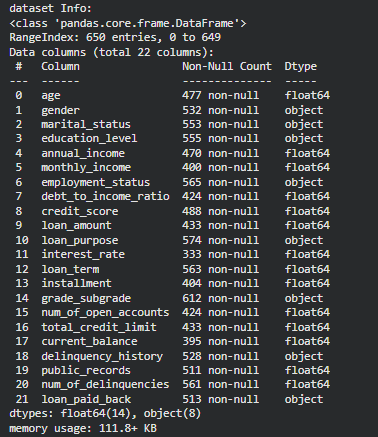
\includegraphics[width=0.4\linewidth]{overview1.png}
\caption{Dataset Information Showing Feature Names, Data Types, and Non-Null Values}
\end{figure}
\textbf{Inference:}
The dataset contains 650 records and 22 features, consisting of both numerical (float64) and categorical (object) attributes.
The non-null count for each feature reveals that several columns contain missing values, indicating the need for data preprocessing.
This overview provides a clear understanding of the dataset's structure and helps determine appropriate preprocessing and feature engineering steps before model training.

\subsection*{Statistical summary}
\begin{figure}[H]
\centering
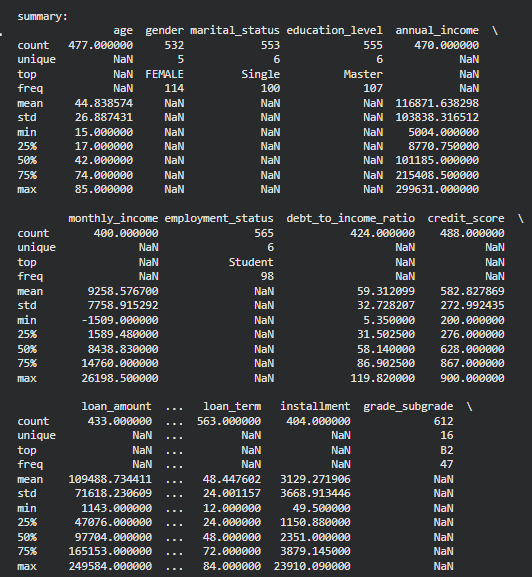
\includegraphics[width=0.4\linewidth]{summary1.png}
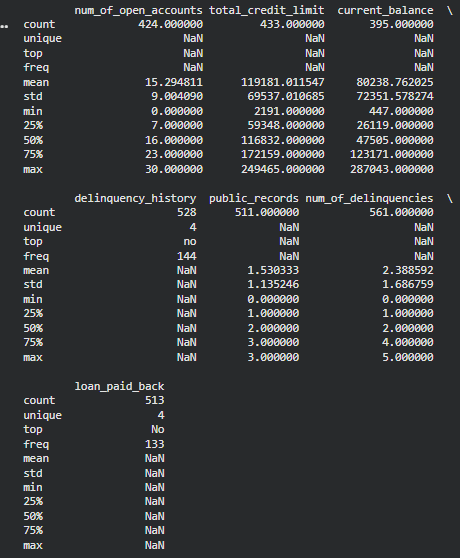
\includegraphics[width=0.4\linewidth]{summary2.png}
\caption{Statistical Summary of the Loan Prediction Dataset}
\end{figure}
\textbf{Inference:}
The statistical summary presents descriptive measures such as count, mean, standard deviation, minimum, maximum, and quartiles for numerical features, along with unique values, most frequent category, and frequency for categorical features.The varying count values indicate that several attributes contain missing values, while the wide ranges in features such as annual income, loan amount, and credit limit suggest high variability in the data.This summary provides an overview of the dataset's distribution and characteristics, helping identify missing data, potential outliers, and the need for preprocessing before model development.

\subsection*{Missing value analysis}
\begin{figure}[H]
\centering
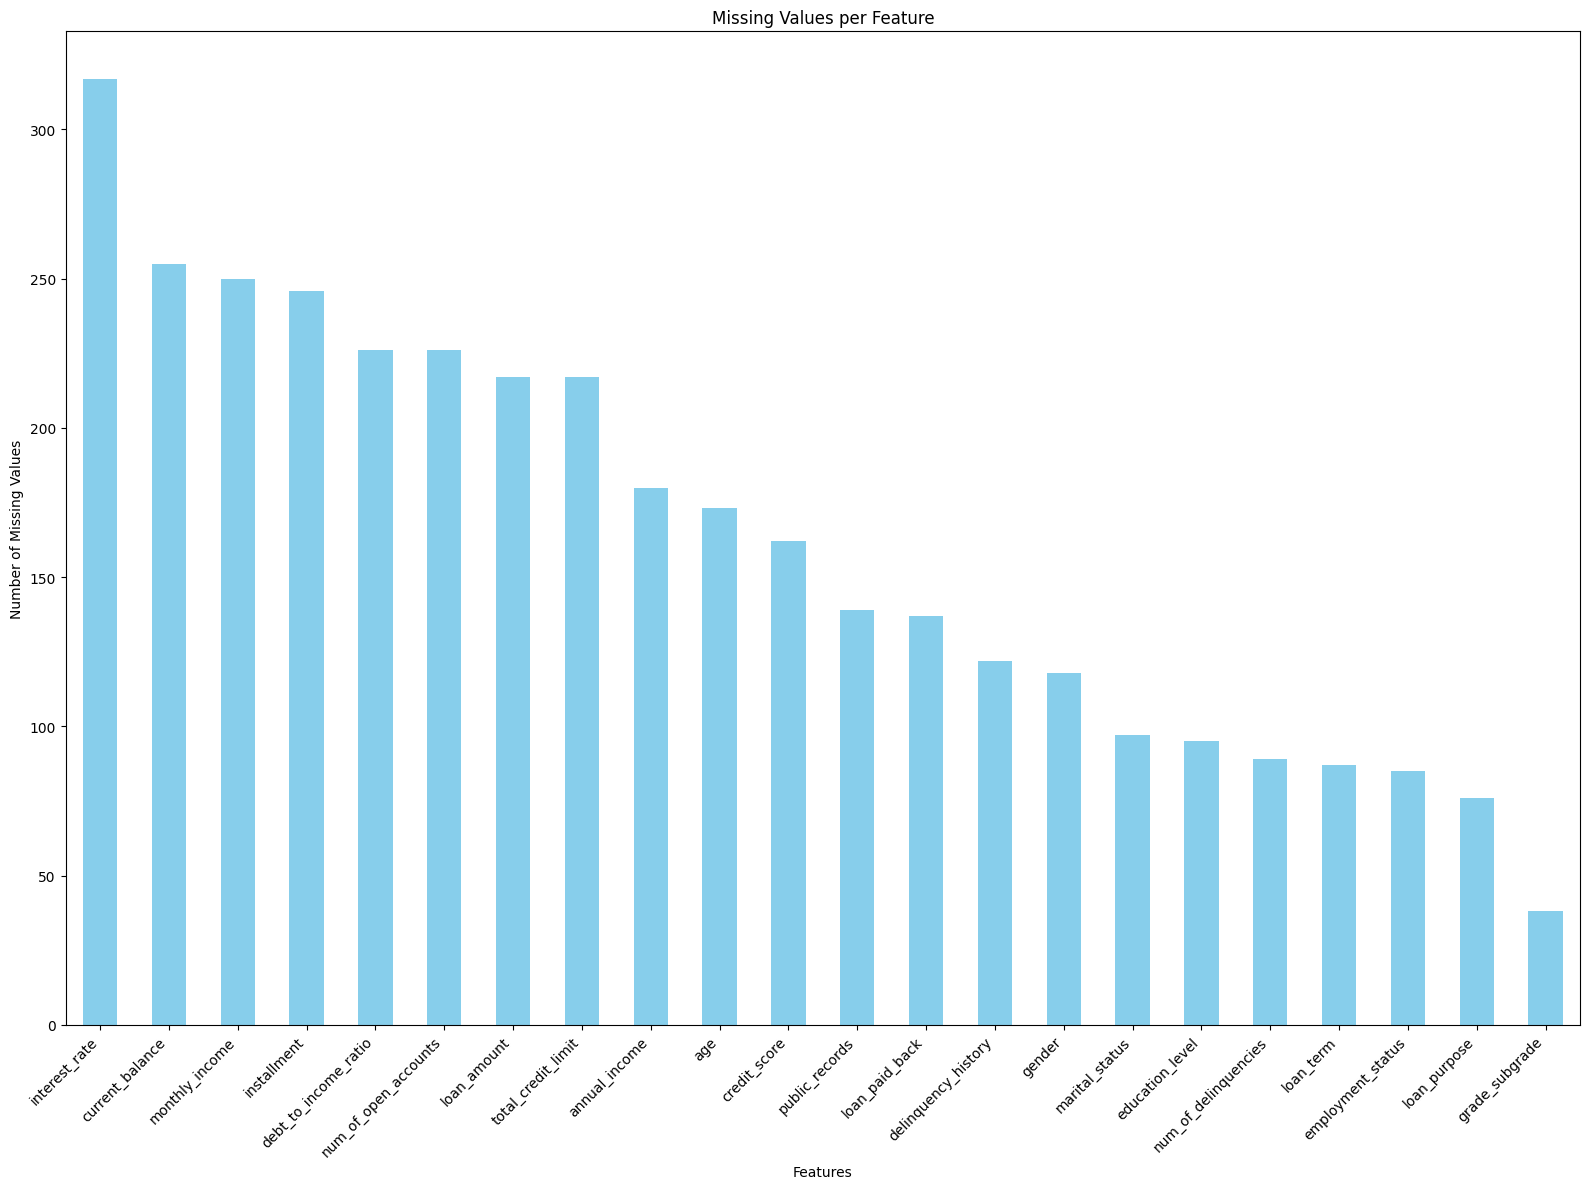
\includegraphics[width=0.4\linewidth]{missing1.png}
\caption{Missing Values Distribution Across Dataset Features}
\end{figure}
\textbf{Inference:}
The graph illustrates the number of missing values present in each feature, highlighting the completeness of the dataset.
Features such as interestrate, currentbalance, and monthlyincome contain the highest number of missing values, whereas gradesubgrade has comparatively fewer missing entries.The presence of missing values across multiple features indicates that appropriate preprocessing techniques, such as imputation or data cleaning, are necessary before model training to ensure reliable analysis.

\subsection*{Class distribution}
\begin{figure}[H]
\centering
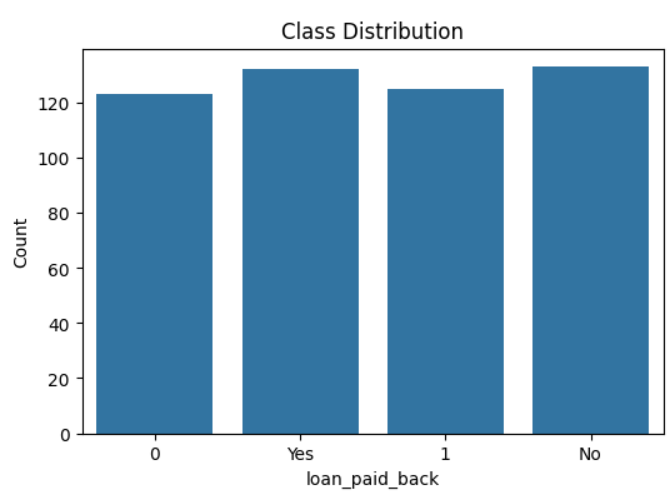
\includegraphics[width=0.4\linewidth]{classd.png}
\caption{Class Distribution of Loan Repayment Status}
\end{figure}
\textbf{Inference:}
The target variable loanpaidback contains four encoded classes with a relatively similar number of samples in each category.
The class distribution is fairly balanced, indicating that no single class dominates the dataset.
A balanced target distribution helps reduce prediction bias and supports reliable classification model training.

\subsection*{Correlation matrix}
\begin{figure}[H]
\centering
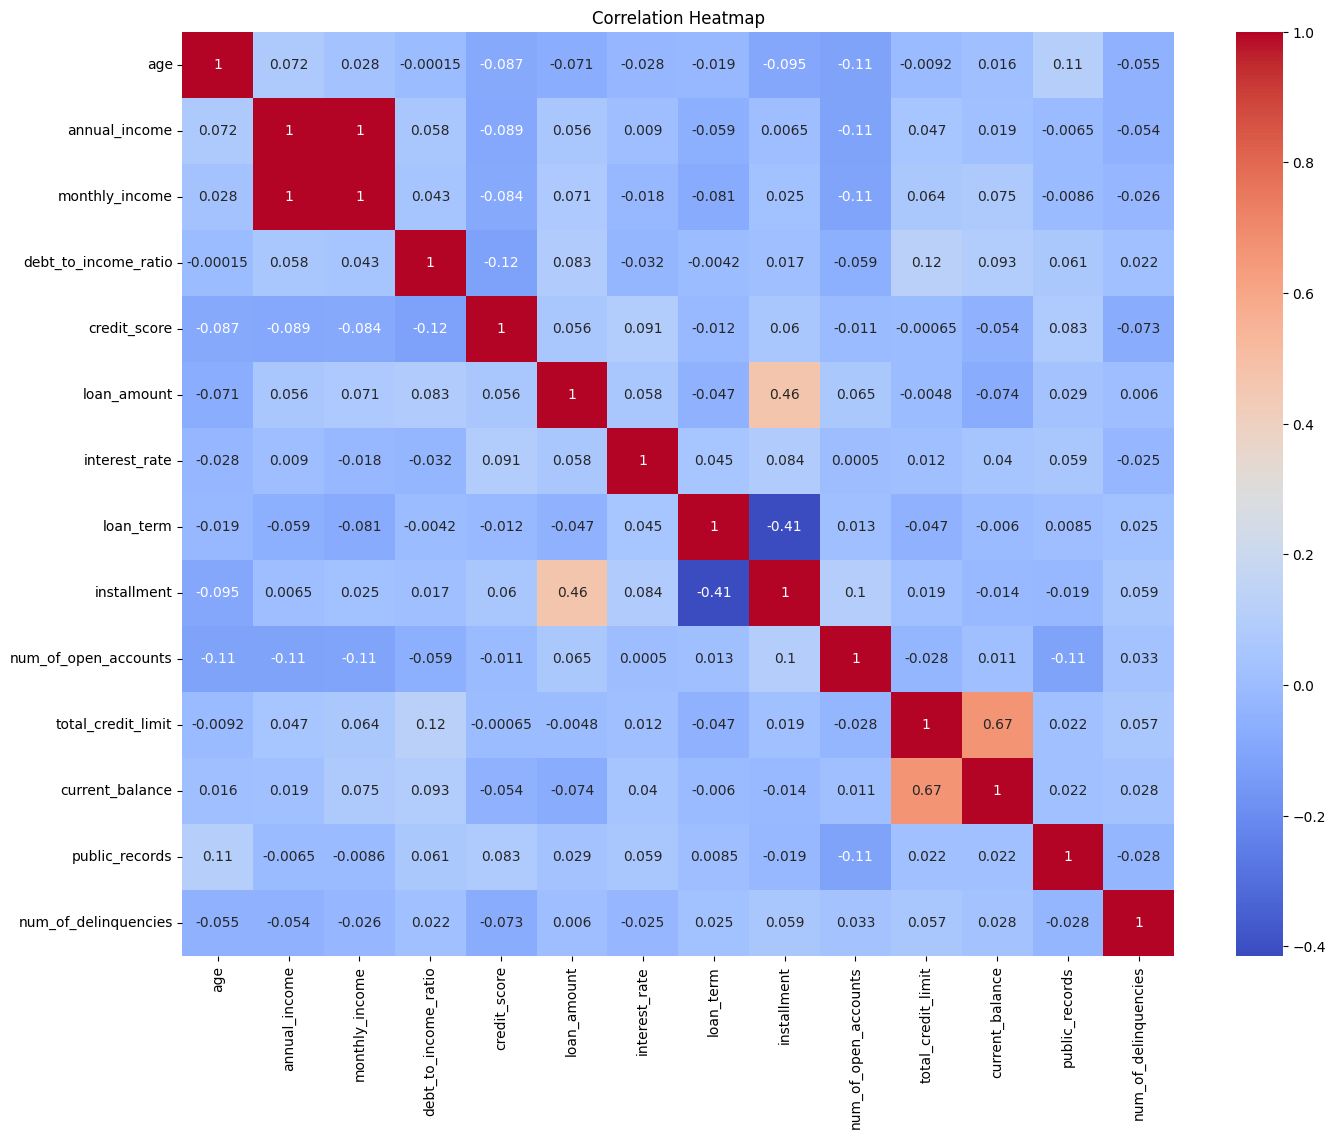
\includegraphics[width=0.4\linewidth]{corr1.png}
\caption{Correlation Heatmap of Numerical Features in the Loan Prediction Dataset}
\end{figure}
\textbf{Inference:}
The heatmap illustrates the correlation coefficients between numerical features, helping identify relationships and potential feature dependencies.
Most feature pairs exhibit weak correlations, indicating that the variables are largely independent and multicollinearity is minimal.
A few feature pairs show moderate to strong correlations, such as annualincome–monthlyincome (1.00), totalcreditlimit–currentbalance (0.67), and loanamount–installment (0.46), which may be considered during feature selection and model building.

\subsection*{Feature distribution}
\begin{figure}[H]
\centering
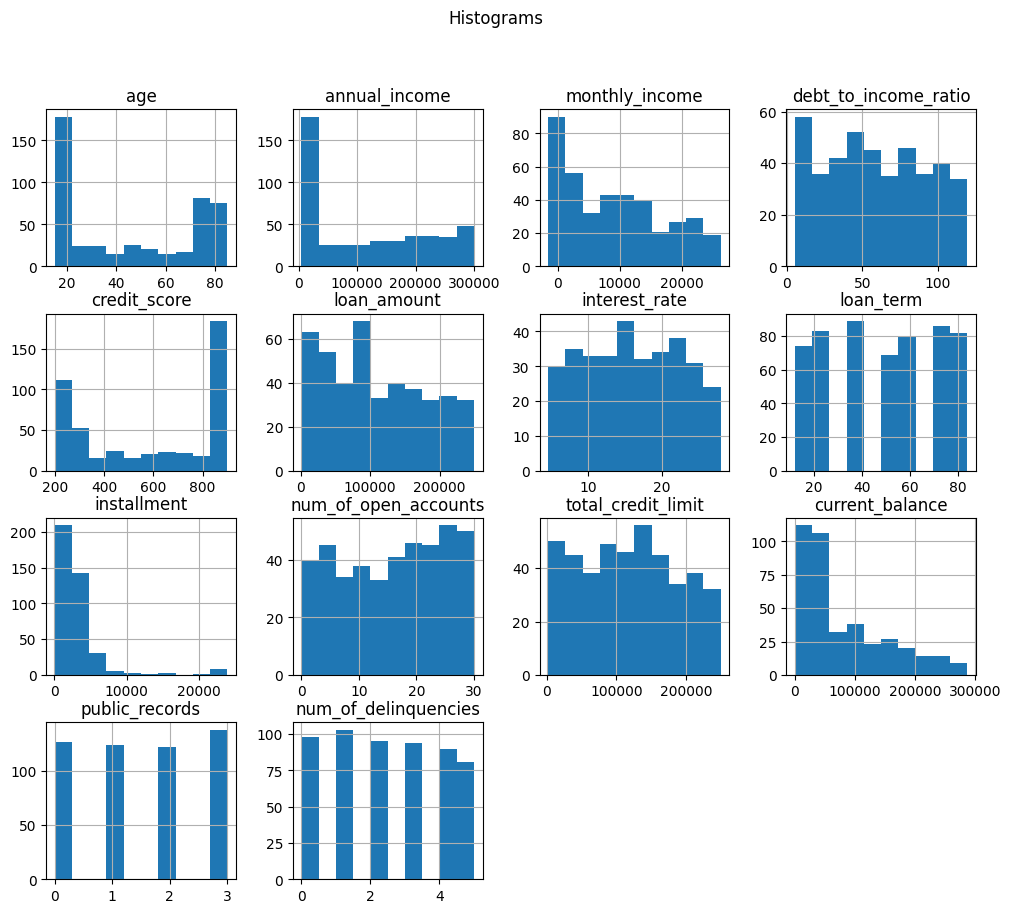
\includegraphics[width=0.4\linewidth]{hist1.png}
\caption{Histogram-Based Distribution of Numerical Features in the Loan Prediction Dataset}
\end{figure}
\textbf{Inference:}
The histograms illustrate the distribution of values for each numerical feature, showing the frequency of observations across different value ranges.
Several features, such as installment, currentbalance, and annualincome, exhibit right-skewed distributions, while others, such as interestrate and debttoincomeratio, appear more evenly distributed.Analyzing these distributions helps identify skewness, potential outliers, and data patterns, which are useful for selecting appropriate preprocessing techniques before model training.
\vspace{0.5cm}
     \item {\Large\textbf{Handwritten character recognition}}
\subsection*{Dataset overview :-}
\begin{figure}[H]
\centering
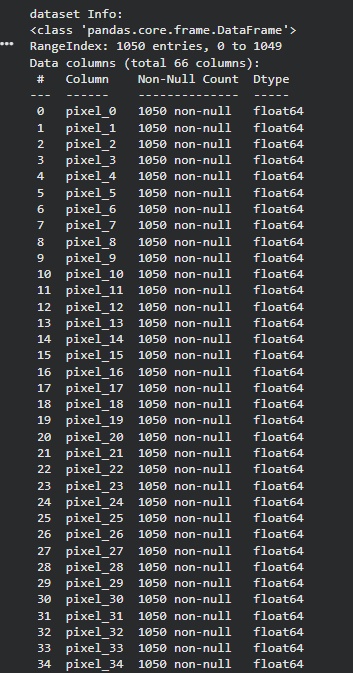
\includegraphics[width=0.4\linewidth]{info2.png}
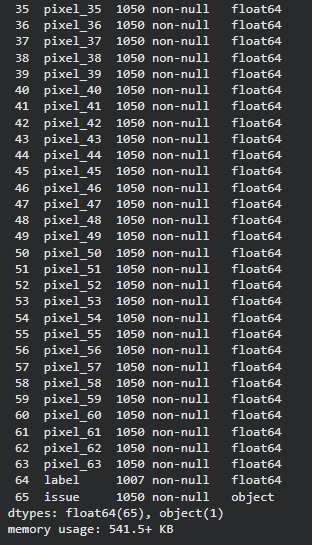
\includegraphics[width=0.4\linewidth]{info22.png}
\caption{Dataset Information Showing Pixel Features, Target Label, and Data Types}
\end{figure}
\textbf{Inference:}
The dataset contains 1,050 samples with 66 columns, comprising 65 numerical pixel features, 1 numerical label column, and 1 categorical issue column.
All pixel features have 1,050 non-null values, indicating that there are no missing values in the dataset.
The pixel values are stored as float64, making them suitable for numerical analysis and machine learning after appropriate preprocessing.

\subsection*{Statistical summary}
\begin{figure}[H]
\centering
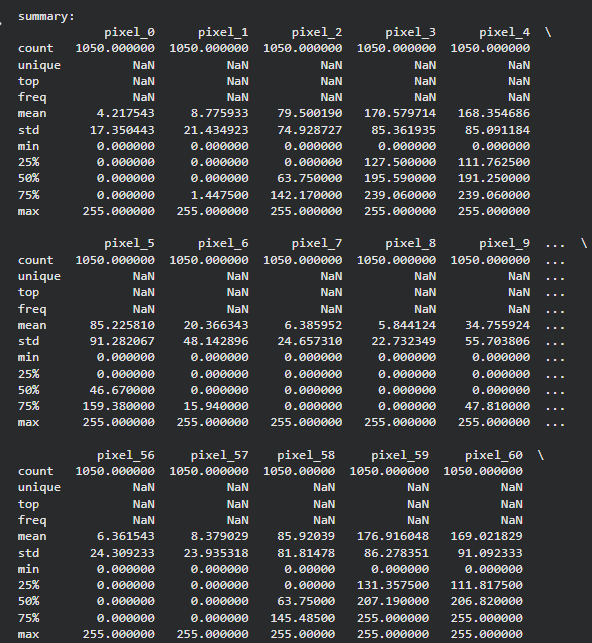
\includegraphics[width=0.4\linewidth]{summary21.png}
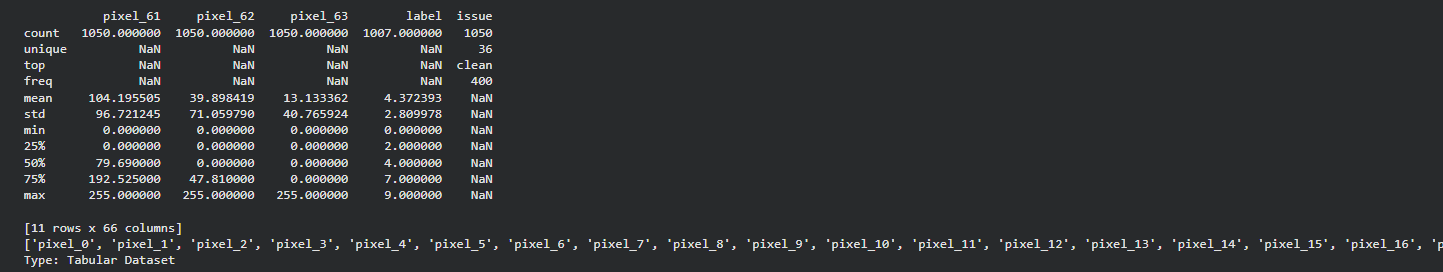
\includegraphics[width=0.4\linewidth]{summary22.png}
\caption{Statistical Summary of Pixel Features and Target Variables in the Handwritten Character Dataset}
\end{figure}
\textbf{Inference:}
The statistical summary shows that the pixel intensity values range from 0 to 255, representing grayscale image data used for handwritten character recognition.
Most pixel features exhibit high variability, indicating diverse handwriting patterns and stroke intensities across the dataset.
The label column contains 1,007 valid entries with character classes ranging from 0 to 9, while the issue column identifies data quality information, with clean being the most frequent category.

\subsection*{Missing value analysis}
\begin{figure}[H]
\centering
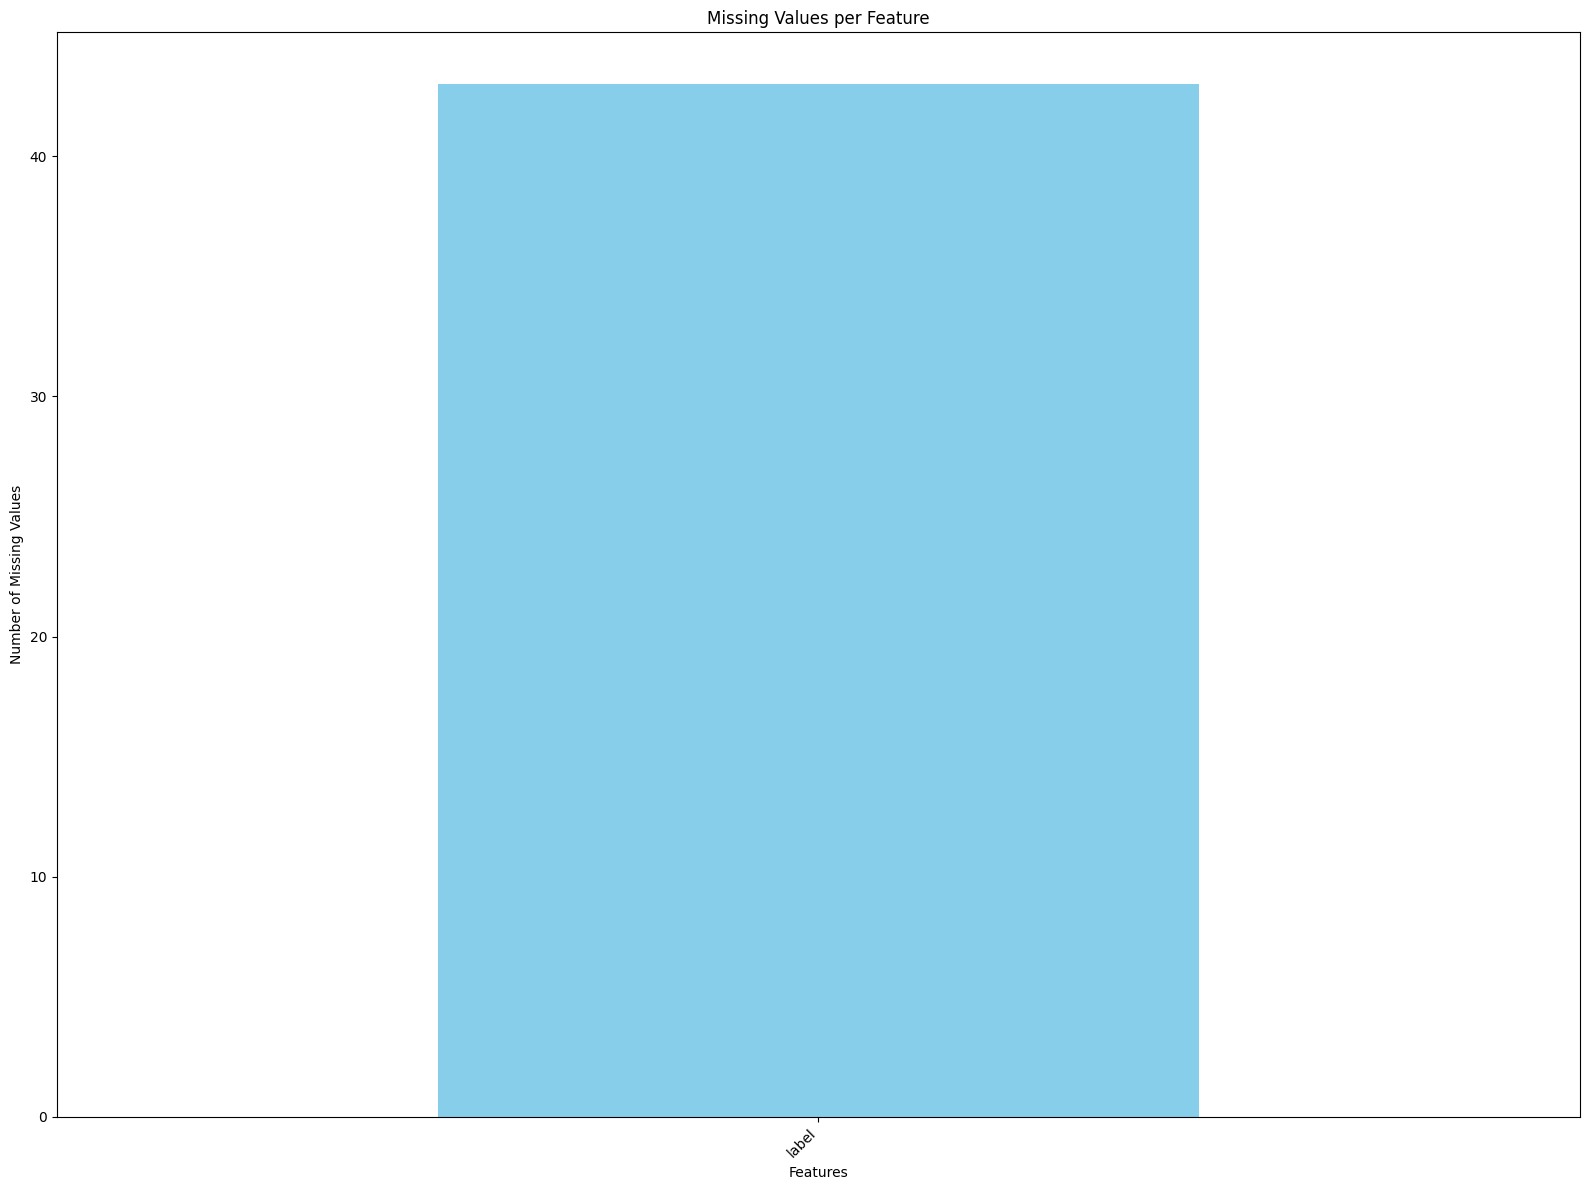
\includegraphics[width=0.4\linewidth]{missing2.png}
\caption{Missing Values Distribution Across Features in the Handwritten Character Dataset}
\end{figure}
\textbf{Inference:}
The graph shows that the label column contains approximately 43 missing values, while all other features have no missing values.
The pixel features are complete, ensuring that the input image data is available for all samples.
The missing values in the label column should be handled through imputation or removal before training the classification model.

\subsection*{Class distribution}
\begin{figure}[H]
\centering
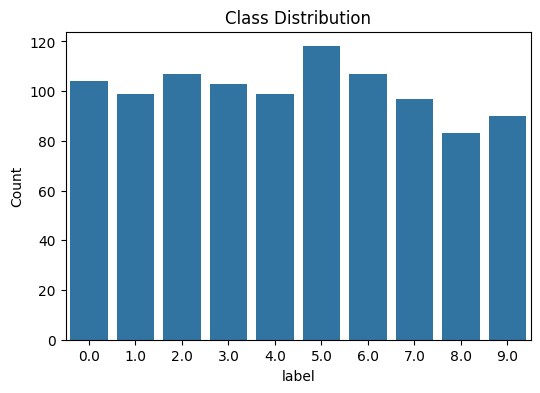
\includegraphics[width=0.4\linewidth]{classd2.png}
\caption{Class Distribution of Handwritten Character Labels}
\end{figure}
\textbf{Inference:}
The dataset contains samples from 10 character classes (0–9), with each class represented by approximately 80–120 samples.
Class 5 has the highest number of samples, while class 8 has the fewest, indicating a slight class imbalance.
Overall, the class distribution is reasonably balanced, making the dataset suitable for training a classification model with minimal bias toward any particular class.

\subsection*{Correlation matrix}
\begin{figure}[H]
\centering
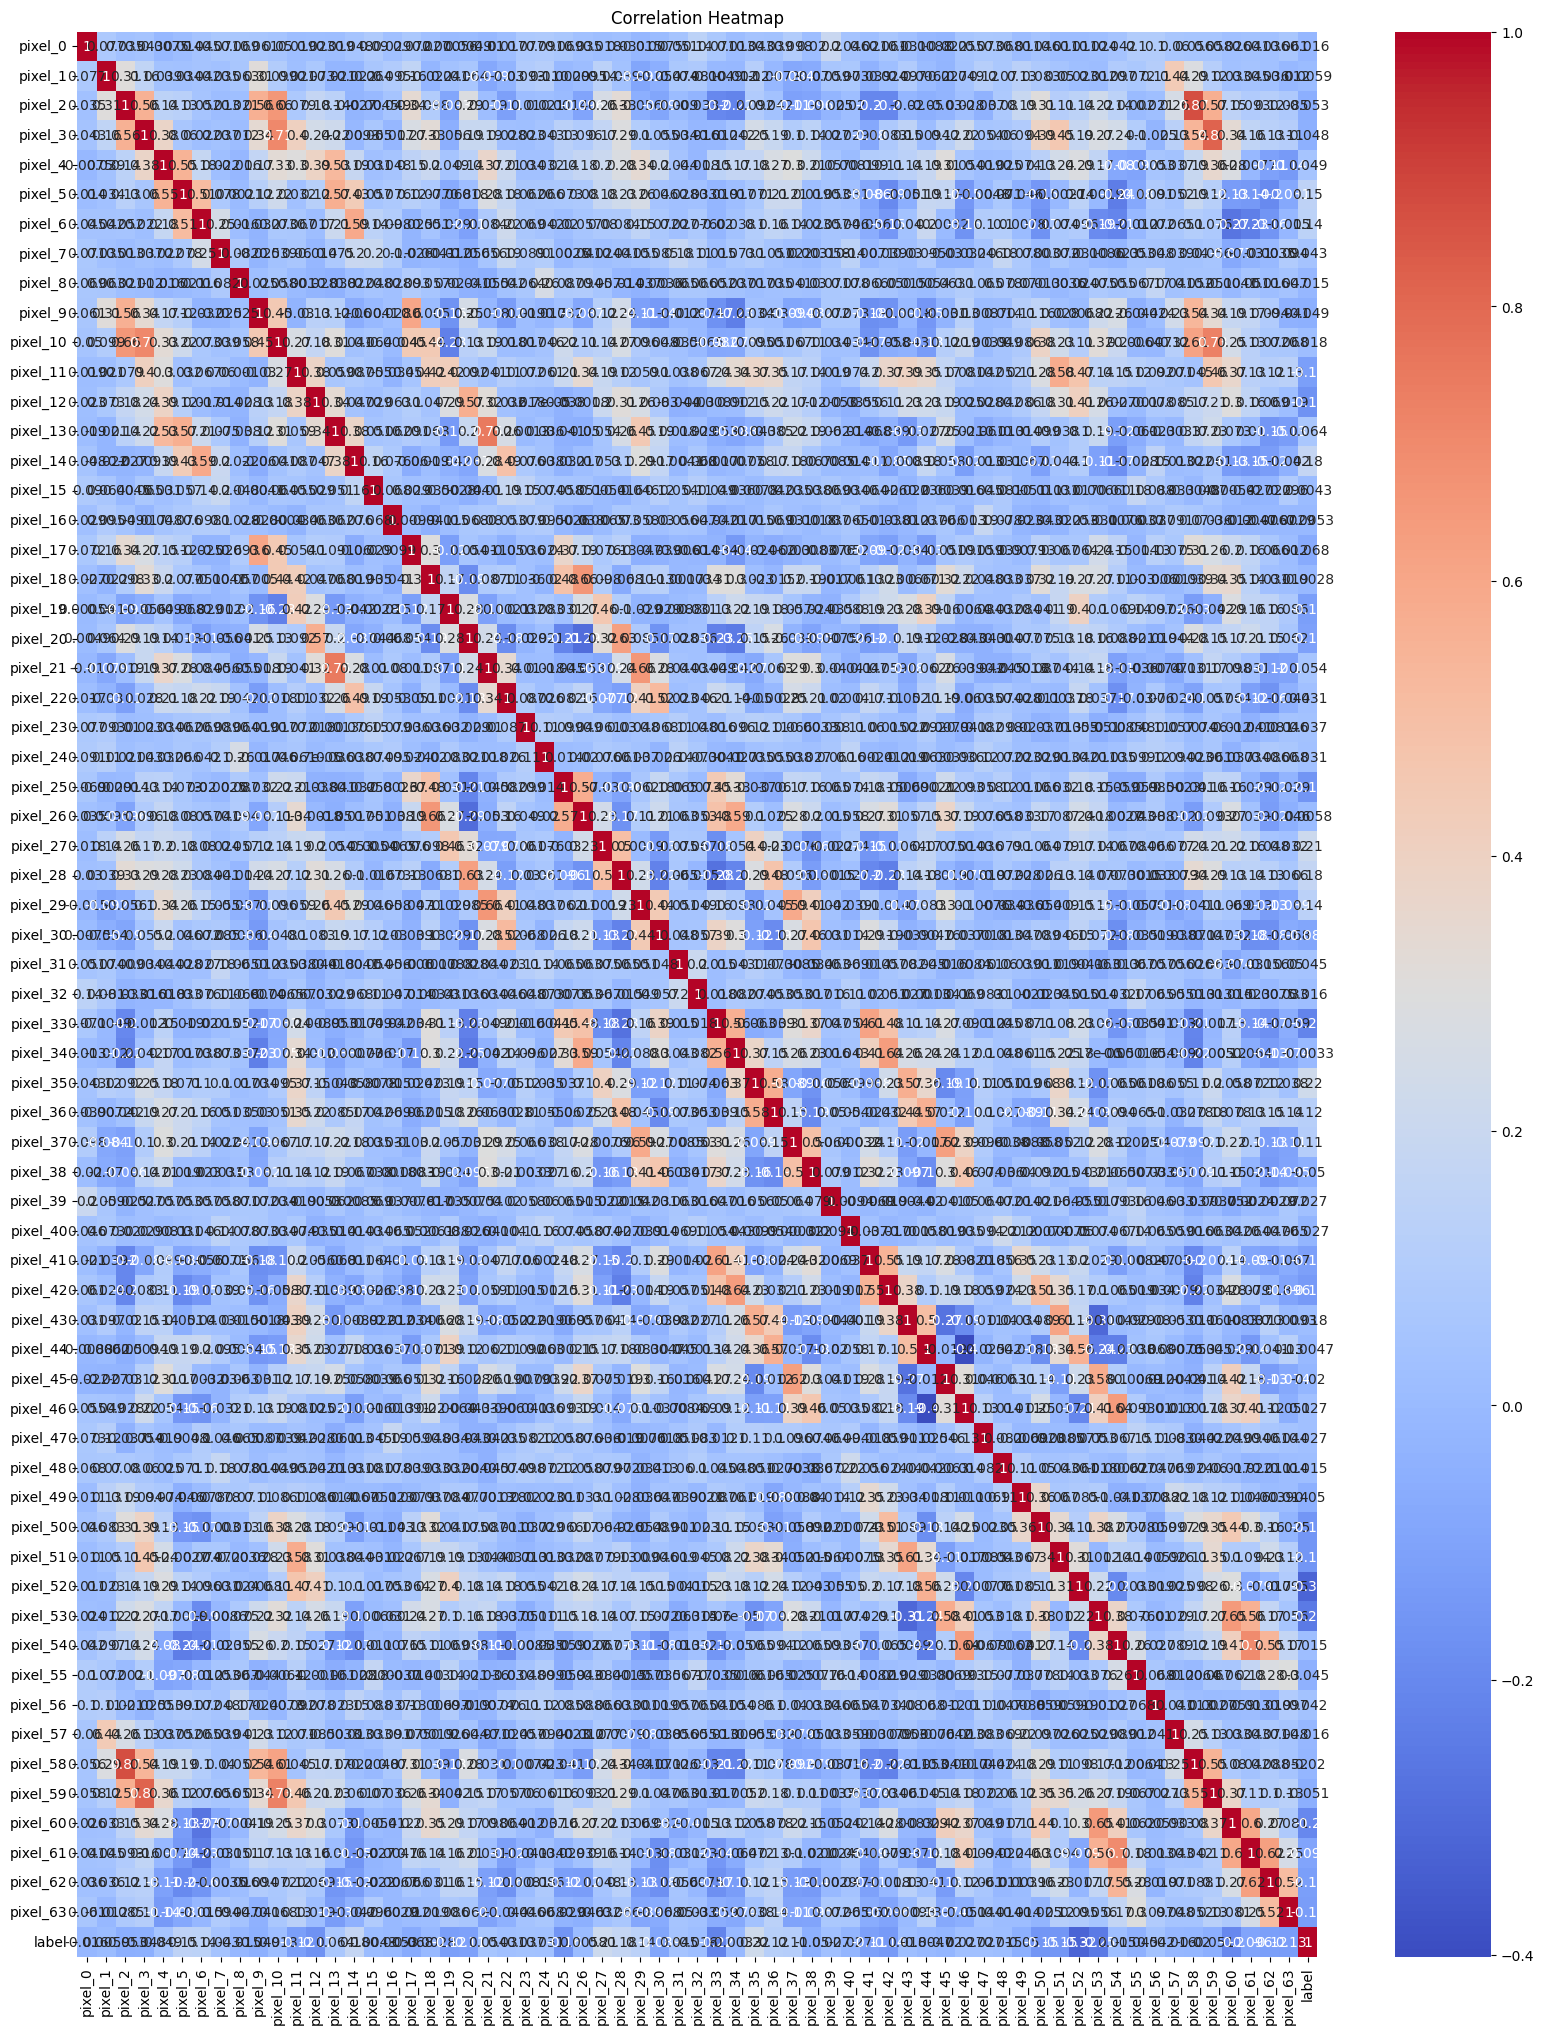
\includegraphics[width=0.4\linewidth]{corr2.png}
\caption{Correlation Heatmap of Pixel Features in the Handwritten Character Dataset}
\end{figure}
\textbf{Inference:}
The heatmap illustrates the pairwise correlation among the 64 pixel features and the target label.
Most pixel features exhibit weak to moderate correlations, indicating that each pixel captures distinct information about the handwritten characters.
The label shows generally low correlation with individual pixel features, suggesting that character recognition depends on the combined pattern of multiple pixels rather than any single feature.

\subsection*{Feature distribution}
\begin{figure}[H]
\centering
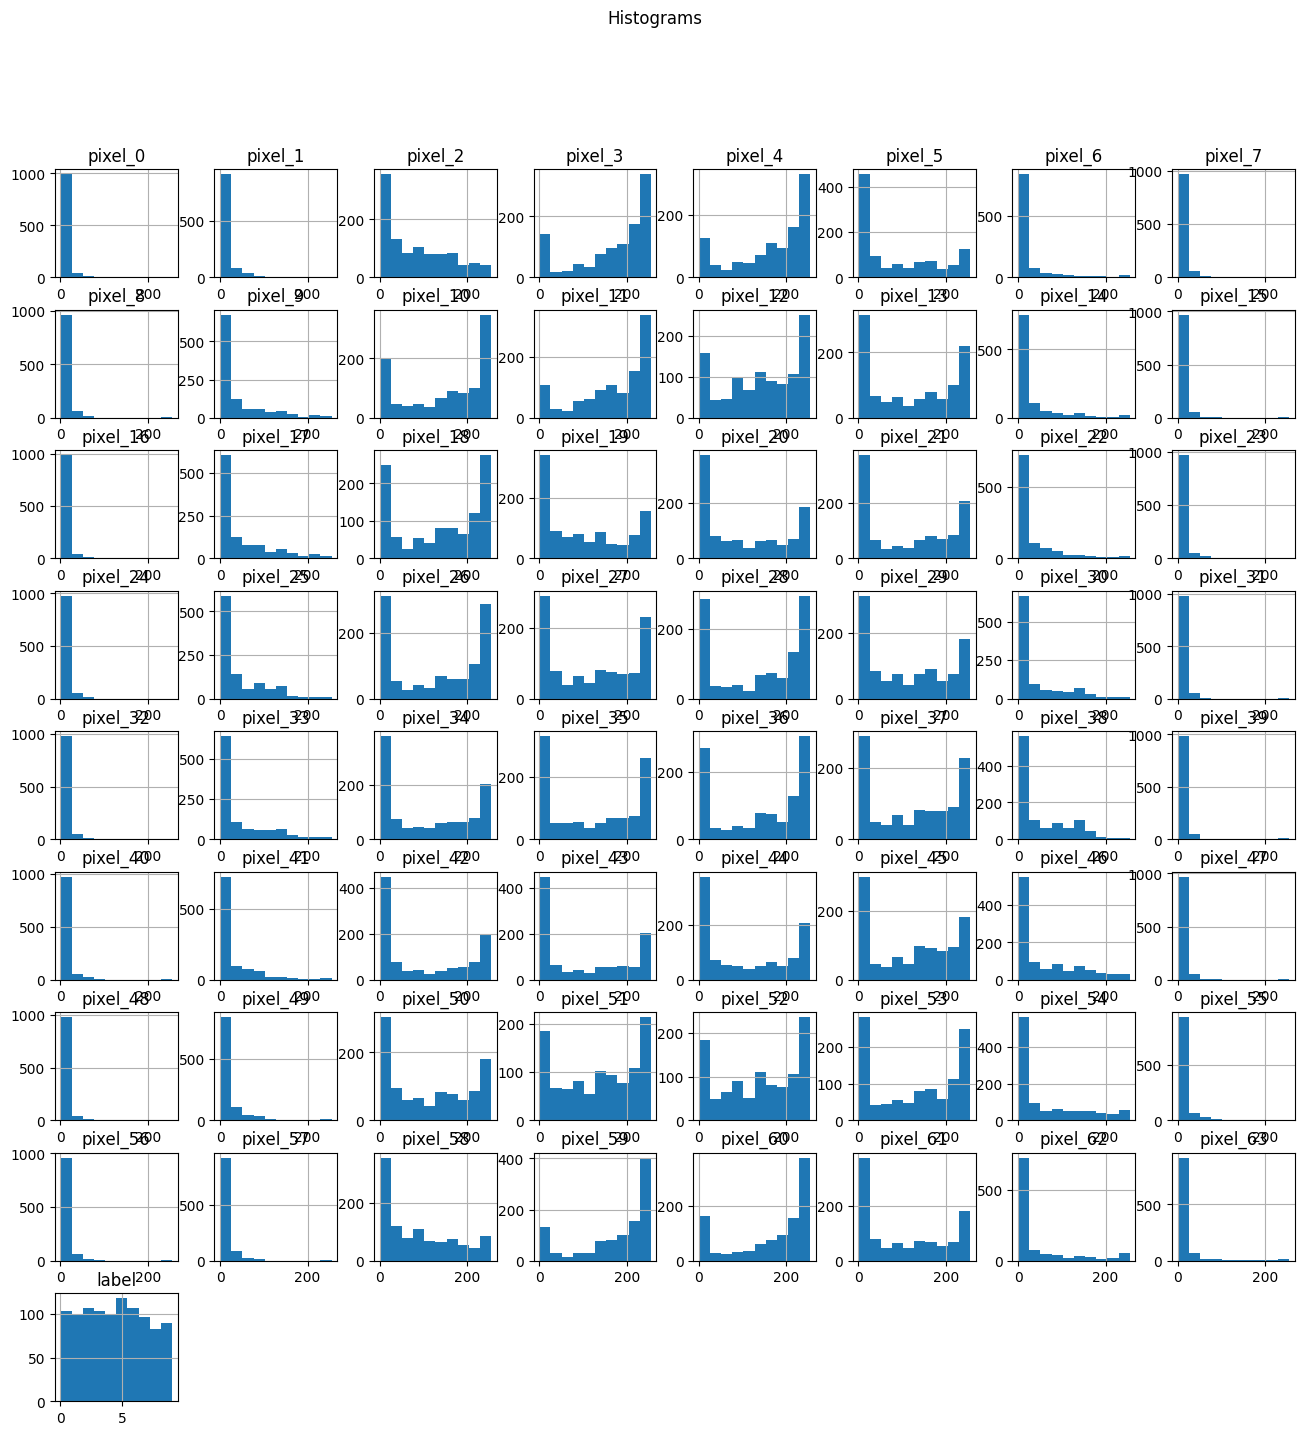
\includegraphics[width=0.4\linewidth]{hist2.png}
\caption{Histogram-Based Distribution of Pixel Intensity Features in the Handwritten Character Dataset}
\end{figure}
\textbf{Inference:}
The histograms illustrate the distribution of pixel intensity values across all 64 pixel features in the dataset.
Many pixel features are highly skewed toward lower intensity values, indicating that a large portion of the image pixels correspond to the background.
Variations in the distributions of different pixel features reflect the diverse stroke patterns and shapes present in handwritten characters.

\vspace{0.5cm}
     \item {\Large\textbf{Classification of Email spam and MNIST data}}
\subsection*{Dataset overview :-}
\begin{figure}[H]
\centering
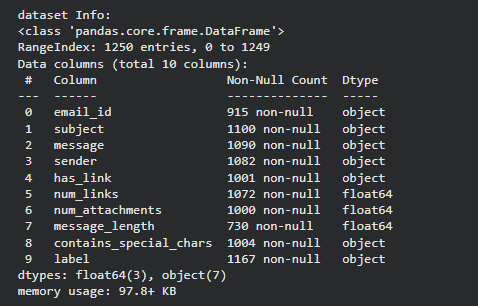
\includegraphics[width=0.4\linewidth]{inf03.png}
\caption{Dataset Information Showing Email Spam Dataset Features, Data Types, and Non-Null Values}
\end{figure}
\textbf{Inference:}
The dataset contains 1,250 email records with 10 features, including both numerical and categorical attributes relevant to spam classification.
Several features, such as emailid, subject, message, sender, and messagelength, contain missing values and require preprocessing before model training.The target label column has 1,167 non-null values, indicating that some records have missing class labels that should be handled before building the classification model.

\subsection*{Statistical summary}
\begin{figure}[H]
\centering
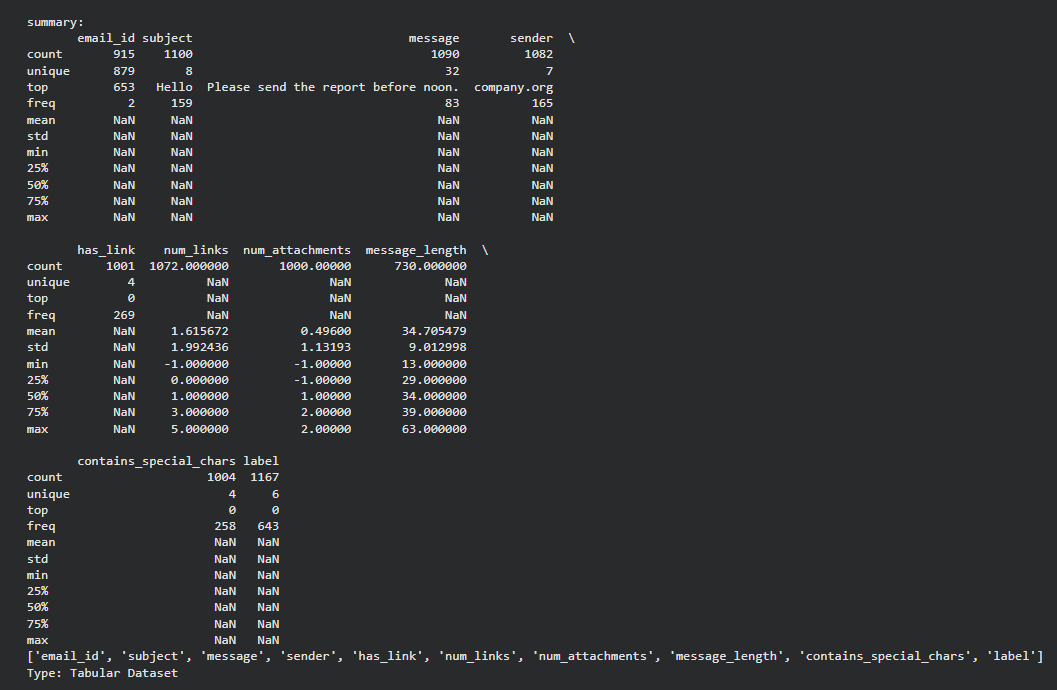
\includegraphics[width=0.4\linewidth]{summary3.png}
\caption{Statistical Summary of the Email Spam Classification Dataset}
\end{figure}
\textbf{Inference:}
he statistical summary presents descriptive statistics for both categorical (e.g., subject, message, sender) and numerical features (e.g., numlinks, numattachments, messagelength).The varying count values across features indicate the presence of missing values, which require preprocessing before model training.The dataset contains diverse email characteristics, such as message length, number of links, attachments, and special characters, which can be used as predictive features for spam classification.

\subsection*{Missing value analysis}
\begin{figure}[H]
\centering
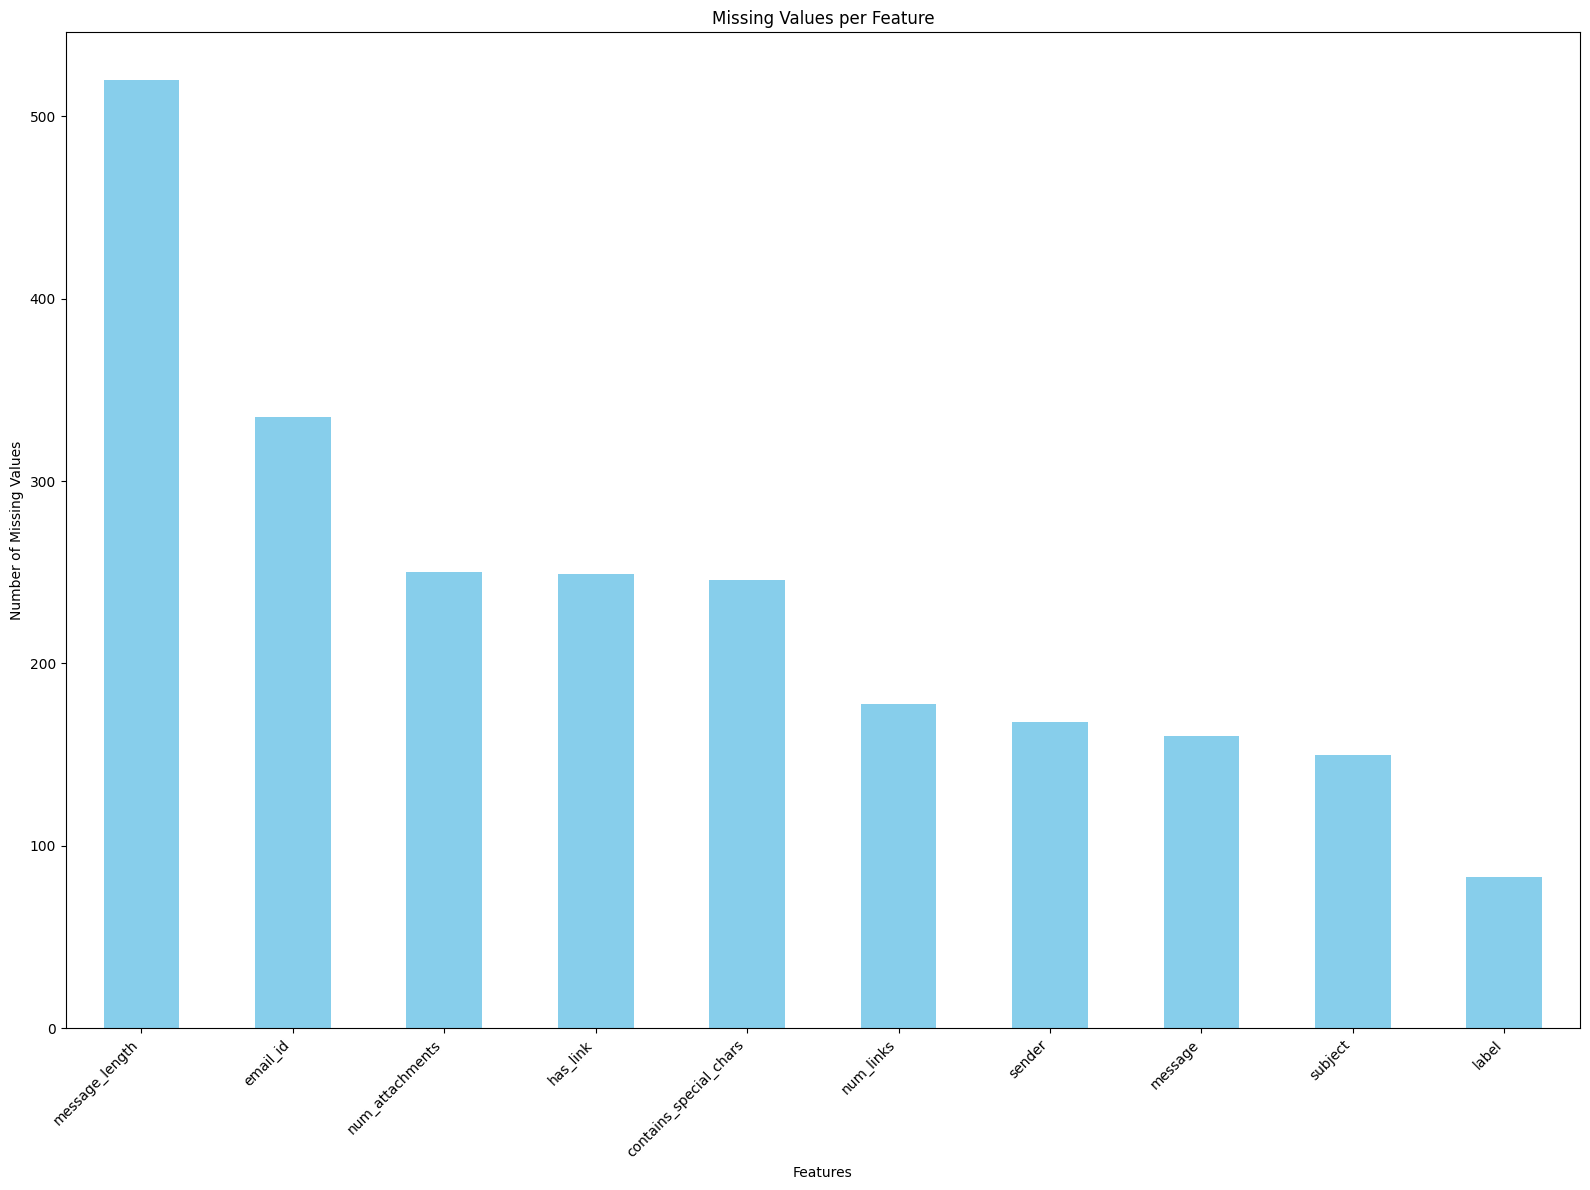
\includegraphics[width=0.4\linewidth]{missing3.png}
\caption{Missing Values Distribution Across Features in the Email Spam Classification Dataset}
\end{figure}
\textbf{Inference:}
The graph shows that several features contain missing values, with messagelength having the highest number of missing entries, followed by emailid.Other features such as numattachments, haslink, containsspecialchars, numlinks, sender, message, subject, and label also contain missing values that require preprocessing.
Proper handling of these missing values through imputation or removal is necessary to improve data quality and ensure reliable spam classification.

\subsection*{Class distribution}
\begin{figure}[H]
\centering
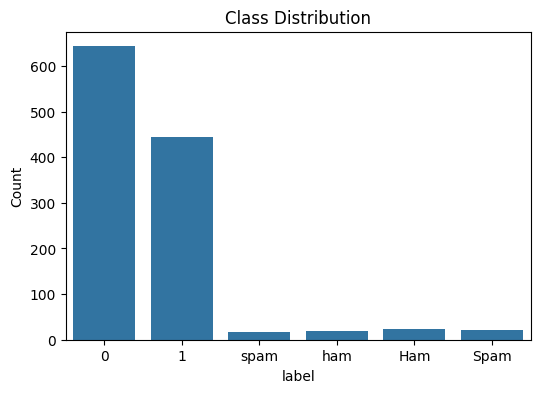
\includegraphics[width=0.4\linewidth]{classd3.png}
\caption{Class Distribution of Email Spam Labels}
\end{figure}
\textbf{Inference:}
The dataset contains multiple representations of the target classes, including 0, 1, spam, ham, Ham, and Spam.The numeric labels (0 and 1) constitute the majority of the samples, while the text-based labels occur less frequently.The presence of inconsistent class labels indicates that the target variable should be standardized (e.g., converting all labels to Spam and Ham or 0 and 1) before training the classification model.

\subsection*{Correlation matrix}
\begin{figure}[H]
\centering
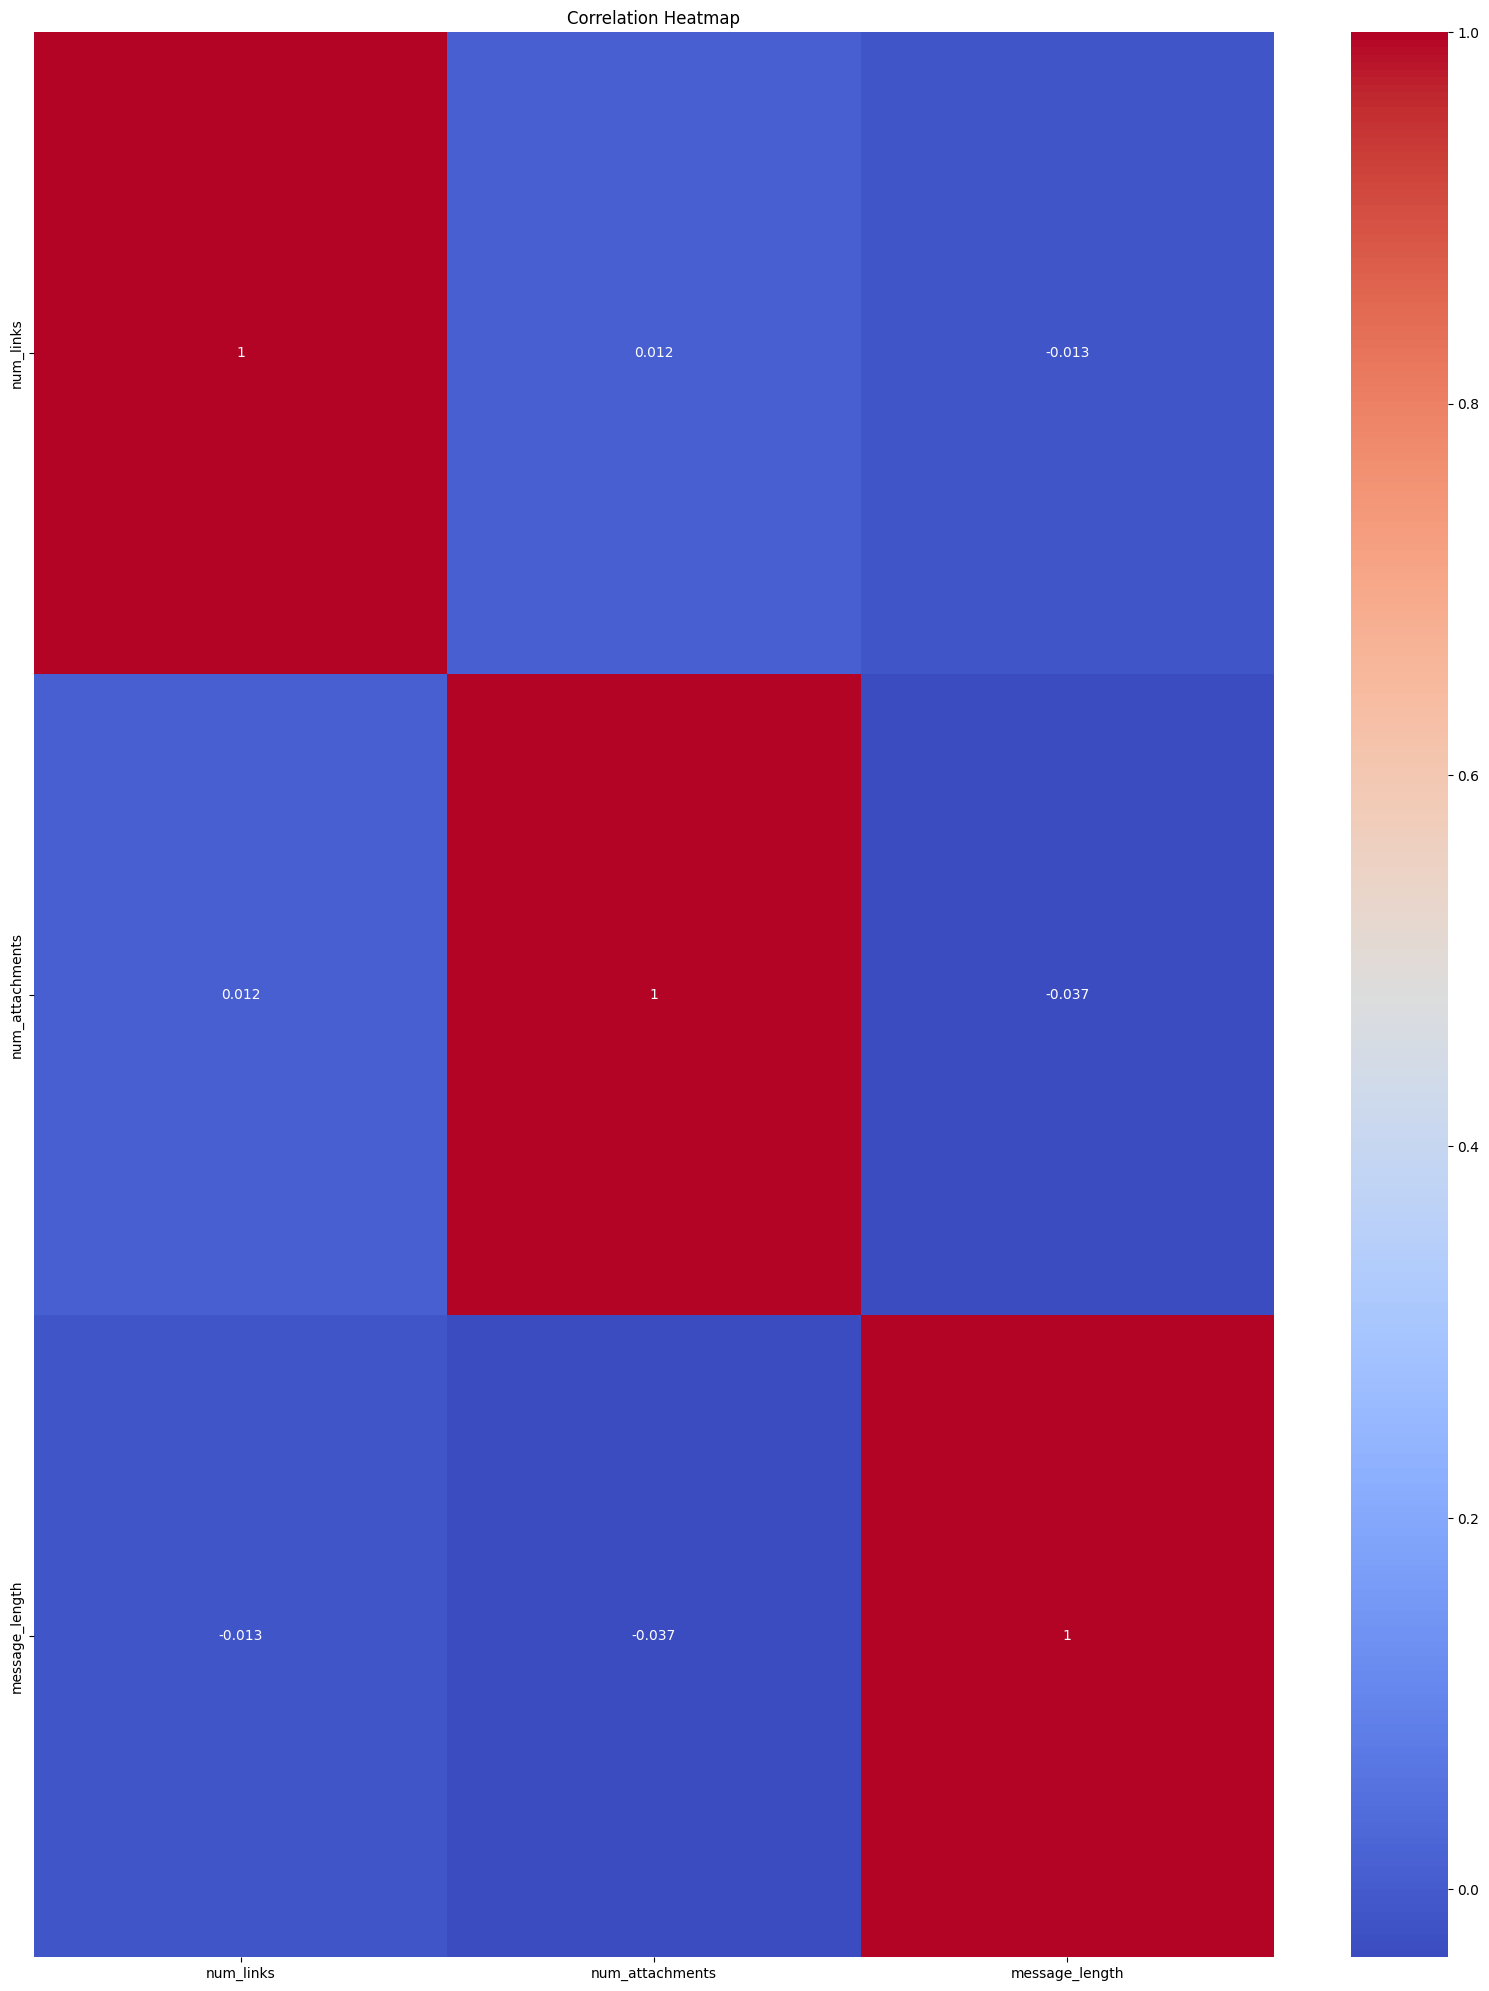
\includegraphics[width=0.4\linewidth]{corr3.png}
\caption{Correlation Heatmap of Numerical Features in the Email Spam Classification Dataset}
\end{figure}
\textbf{Inference:}
The heatmap shows the pairwise correlations among the numerical features numlinks, numattachments, and messagelength.All feature pairs exhibit very weak correlations (correlation coefficients close to 0), indicating that these features are largely independent of one another.The absence of strong correlations suggests that each numerical feature contributes distinct information for email spam classification.

\subsection*{Feature distribution}
\begin{figure}[H]
\centering
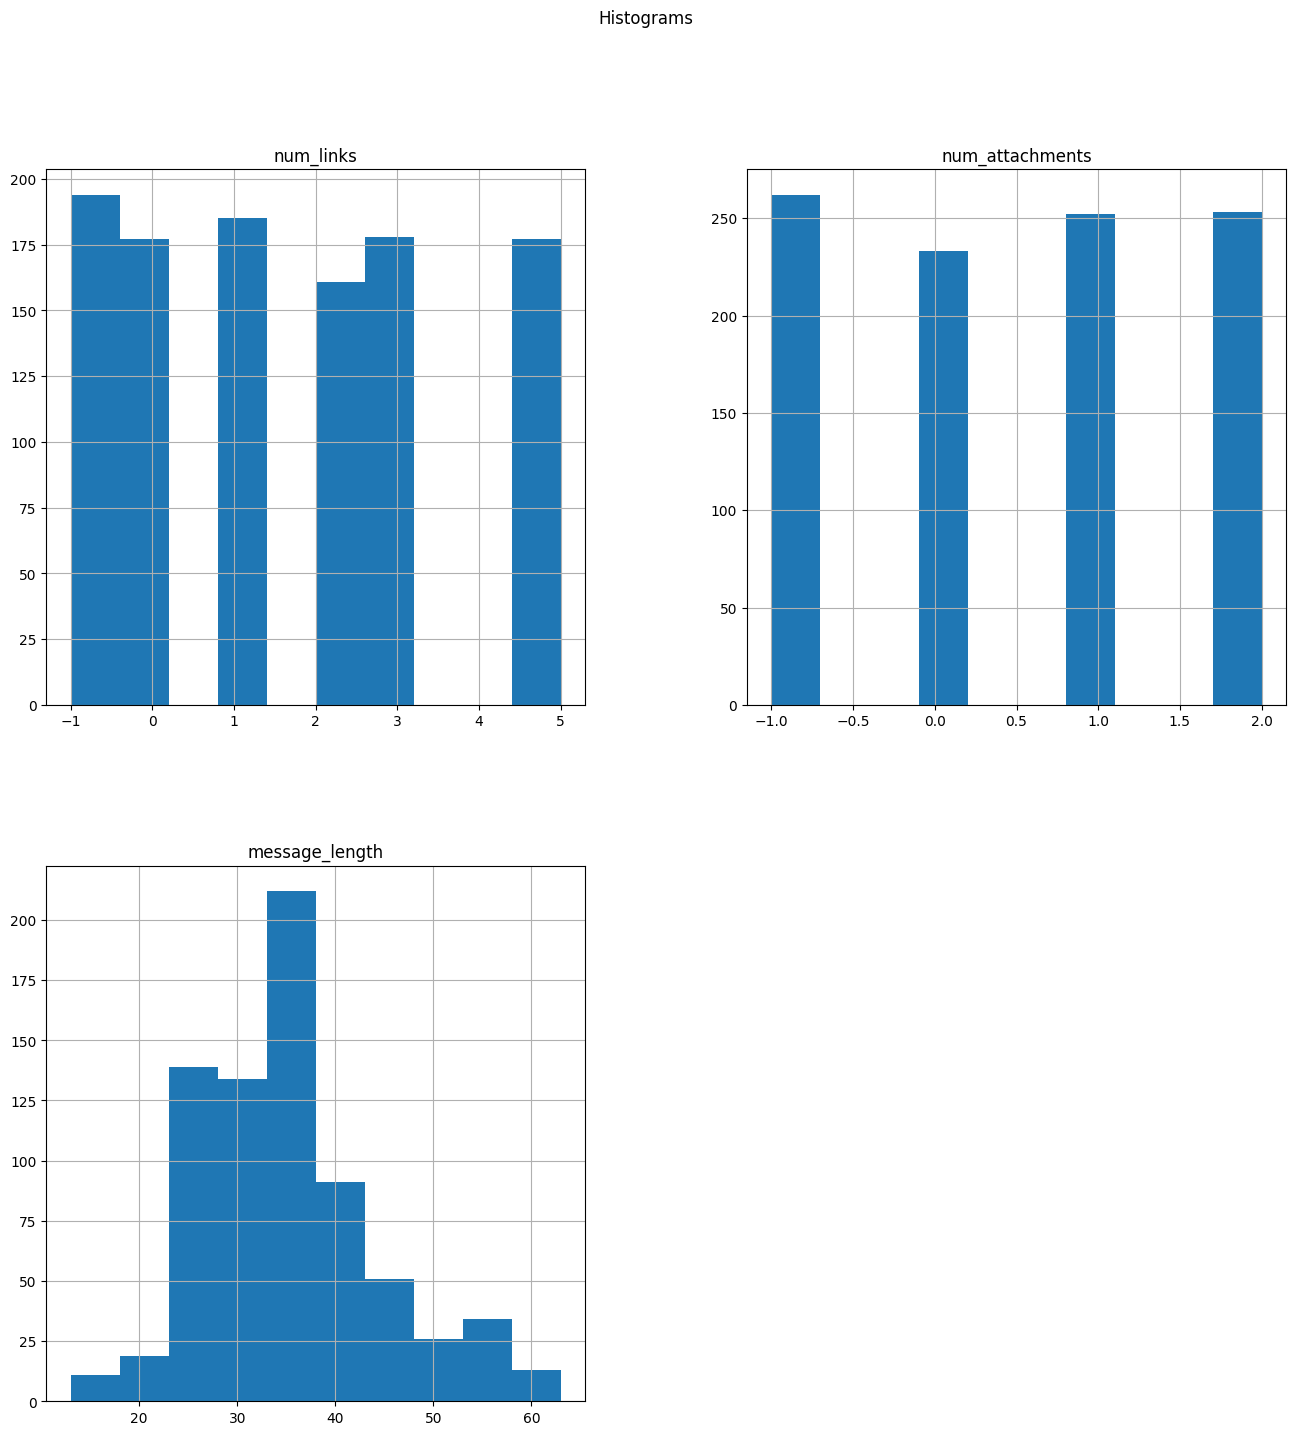
\includegraphics[width=0.4\linewidth]{hist3.png}
\caption{Histogram-Based Distribution of Numerical Features in the Email Spam Classification Dataset}
\end{figure}
\textbf{Inference:}
The histograms illustrate the distributions of the numerical features numlinks, numattachments, and messagelength.messagelength exhibits a broader spread with most emails containing approximately 25–40 characters, while numlinks and numattachments are concentrated around a few discrete values.
The varying distributions indicate that these numerical features capture different characteristics of emails and can contribute useful information for spam classification.
\vspace{0.5cm}
     \item {\Large\textbf{Predicting Diabetes}}
\subsection*{Dataset overview :-}
\begin{figure}[H]
\centering
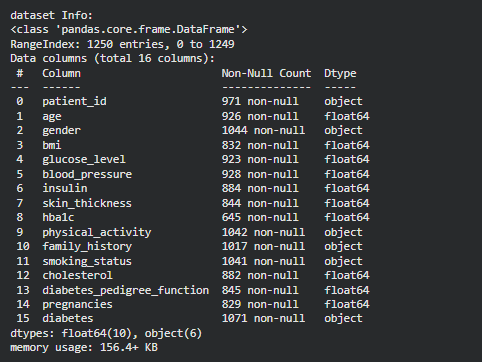
\includegraphics[width=0.4\linewidth]{overview4.png}
\caption{Dataset Information Showing Feature Names, Data Types, and Non-Null Values of the Diabetes Prediction Dataset}
\end{figure}
\textbf{Inference:}
The dataset contains 1,250 records with 16 features, comprising 10 numerical and 6 categorical attributes related to patient health and diabetes risk.
Several features contain missing values, with hba1c (645 non-null) having the highest number of missing entries, followed by bmi, pregnancies, and cholesterol, indicating that preprocessing is required.The target variable diabetes has 1,071 non-null values and is categorical (object), making the dataset suitable for a supervised classification task after handling missing values and encoding categorical features.

\subsection*{Statistical summary}
\begin{figure}[H]
\centering
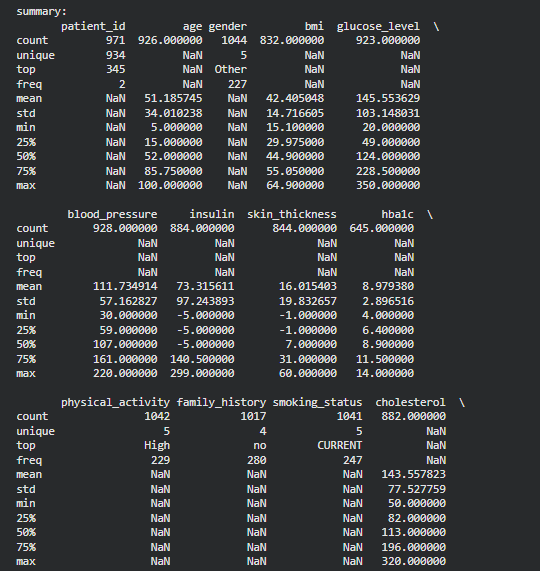
\includegraphics[width=0.4\linewidth]{summary41.png}
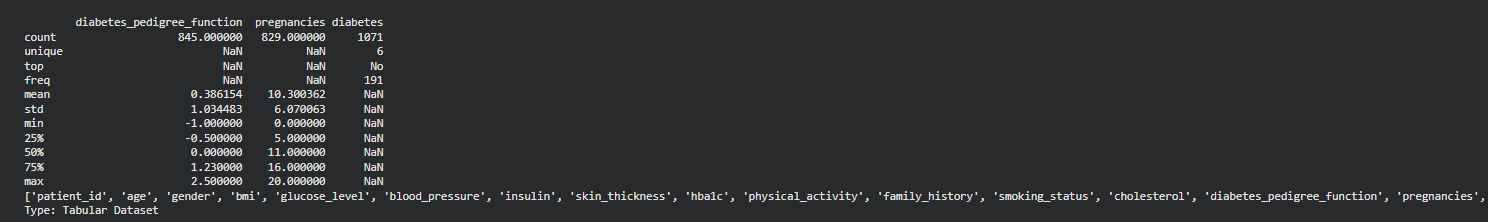
\includegraphics[width=0.4\linewidth]{summary42.png}
\caption{Statistical Summary of the Diabetes Prediction Dataset}
\end{figure}
\textbf{Inference:}
The statistical summary provides descriptive measures such as count, mean, standard deviation, minimum, maximum, and quartiles for numerical features, along with unique values and frequency for categorical features.
The dataset contains a mix of continuous variables (e.g., age, BMI, glucose level, blood pressure, cholesterol) and categorical variables (e.g., gender, physical activity, family history, smoking status, diabetes), indicating that different preprocessing techniques are required.
Several features have non-null counts lower than 1,250, confirming the presence of missing values, while the wide ranges of numerical attributes (e.g., glucose level: 20–350, cholesterol: 50–320) indicate substantial variation among patient records.

\subsection*{Missing value analysis}
\begin{figure}[H]
\centering
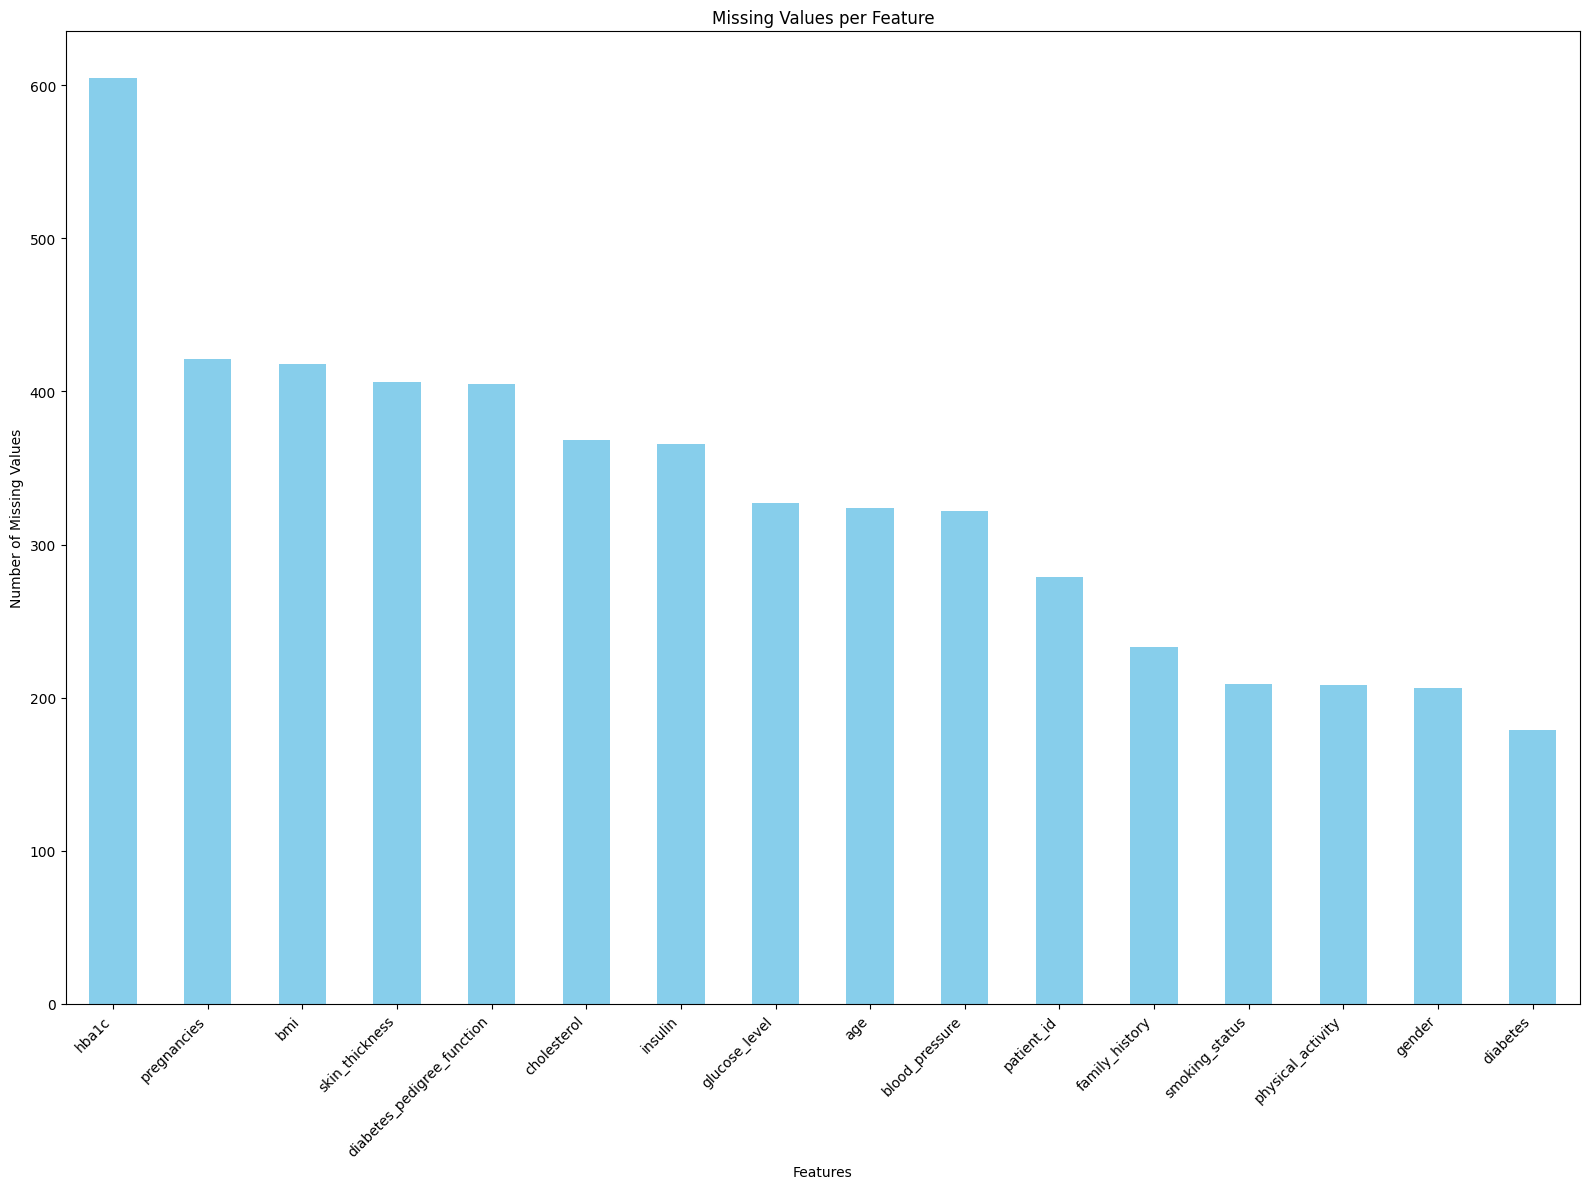
\includegraphics[width=0.4\linewidth]{missing4.png}
\caption{Missing Values Distribution Across Features in the Diabetes Prediction Dataset}
\end{figure}
\textbf{Inference:}
Missing values are present in all features, indicating that data preprocessing is necessary before model training.
The hba1c feature has the highest number of missing values, followed by pregnancies, bmi, and skin\_thickness, making them the most affected attributes.The diabetes target column has the fewest missing values compared to the other features, while the remaining health-related attributes contain moderate levels of missing data that should be handled through appropriate imputation techniques.

\subsection*{Class distribution}
\begin{figure}[H]
\centering
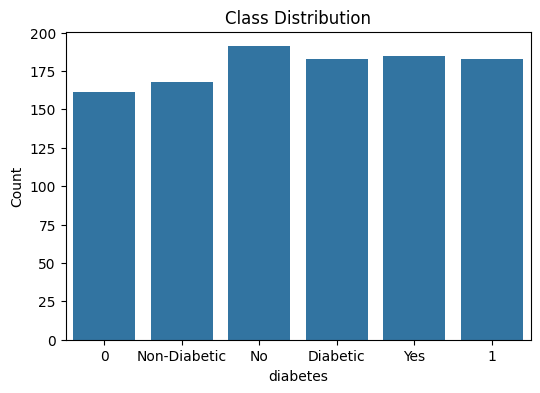
\includegraphics[width=0.4\linewidth]{classd4.png}
\caption{Class Distribution of the Diabetes Prediction Dataset}
\end{figure}
\textbf{Inference:}
The target variable contains six label categories: 0, 1, No, Yes, Non-Diabetic, and Diabetic, indicating inconsistent class labels.
The frequencies of the six classes are relatively similar, with no single class overwhelmingly dominating the dataset.
Before training a classification model, the class labels should be standardized (e.g., mapping 0/No/Non-Diabetic to one class and 1/Yes/Diabetic to the other) to ensure a consistent binary target variable.

\subsection*{Correlation matrix}
\begin{figure}[H]
\centering
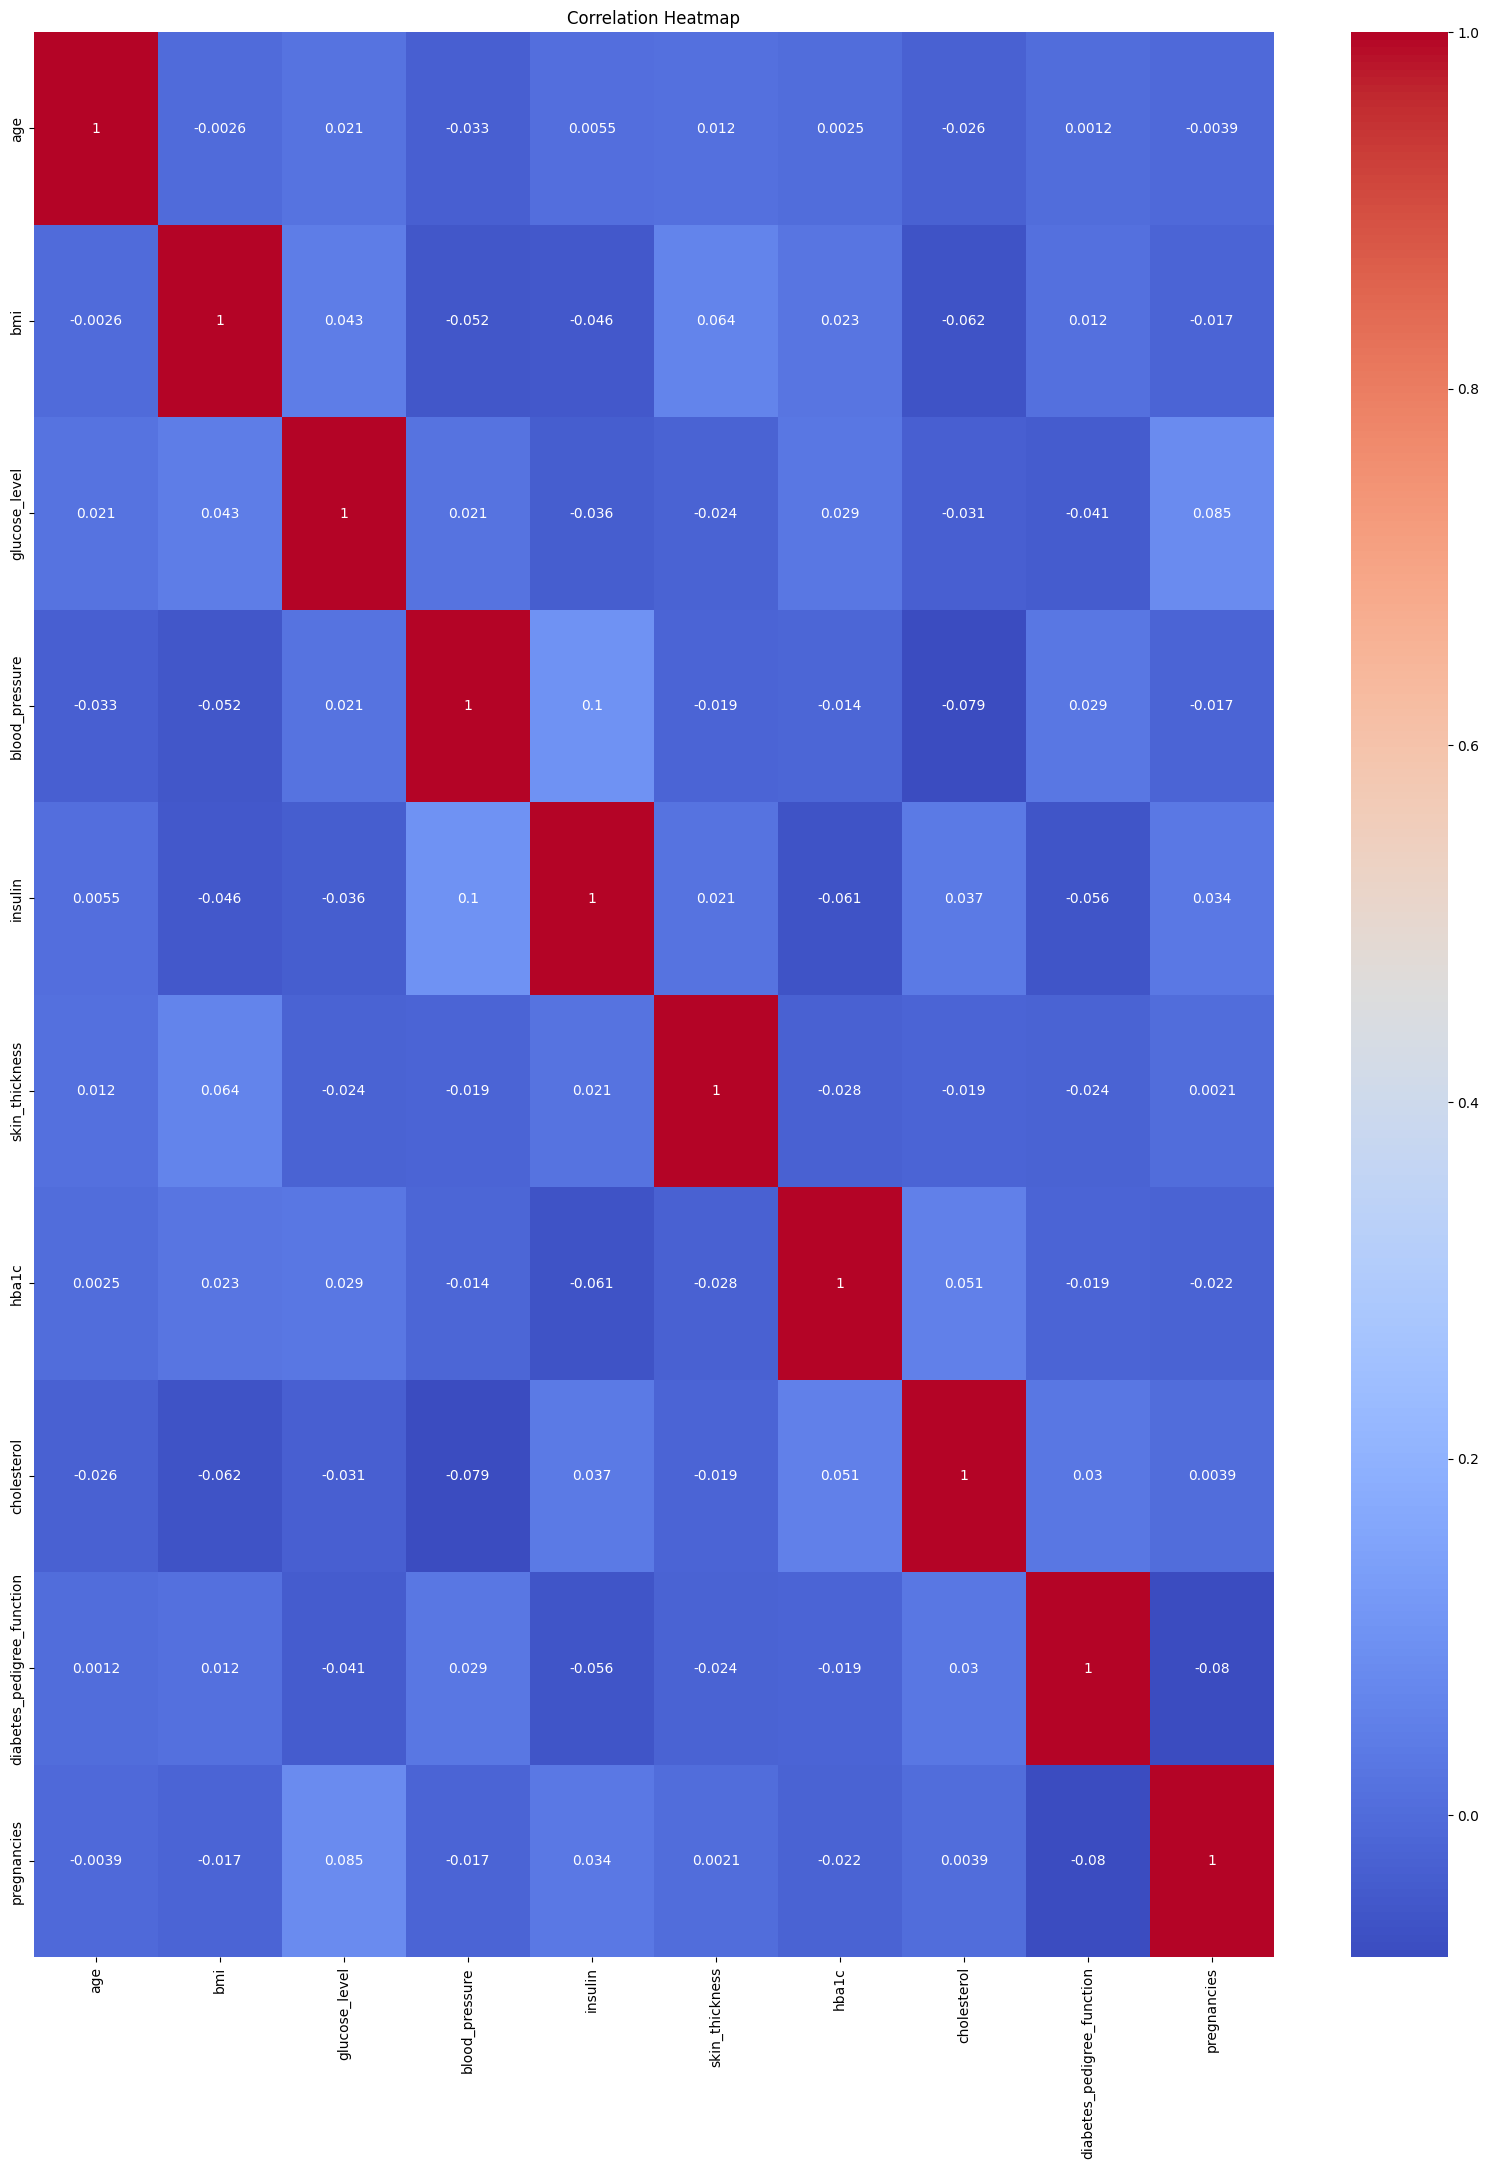
\includegraphics[width=0.4\linewidth]{corr4.png}
\caption{Correlation Heatmap of Numerical Features in the Diabetes Prediction Dataset}
\end{figure}
\textbf{Inference:}
The heatmap shows the pairwise correlations among the numerical features, with diagonal values of 1.0 representing each feature's correlation with itself.Most correlation coefficients are close to zero (approximately -0.1 to 0.1), indicating weak linear relationships between the features and low multicollinearity.The absence of strong positive or negative correlations suggests that the numerical features provide largely independent information, making them useful for diabetes prediction without significant redundancy.

\subsection*{Feature distribution}
\begin{figure}[H]
\centering
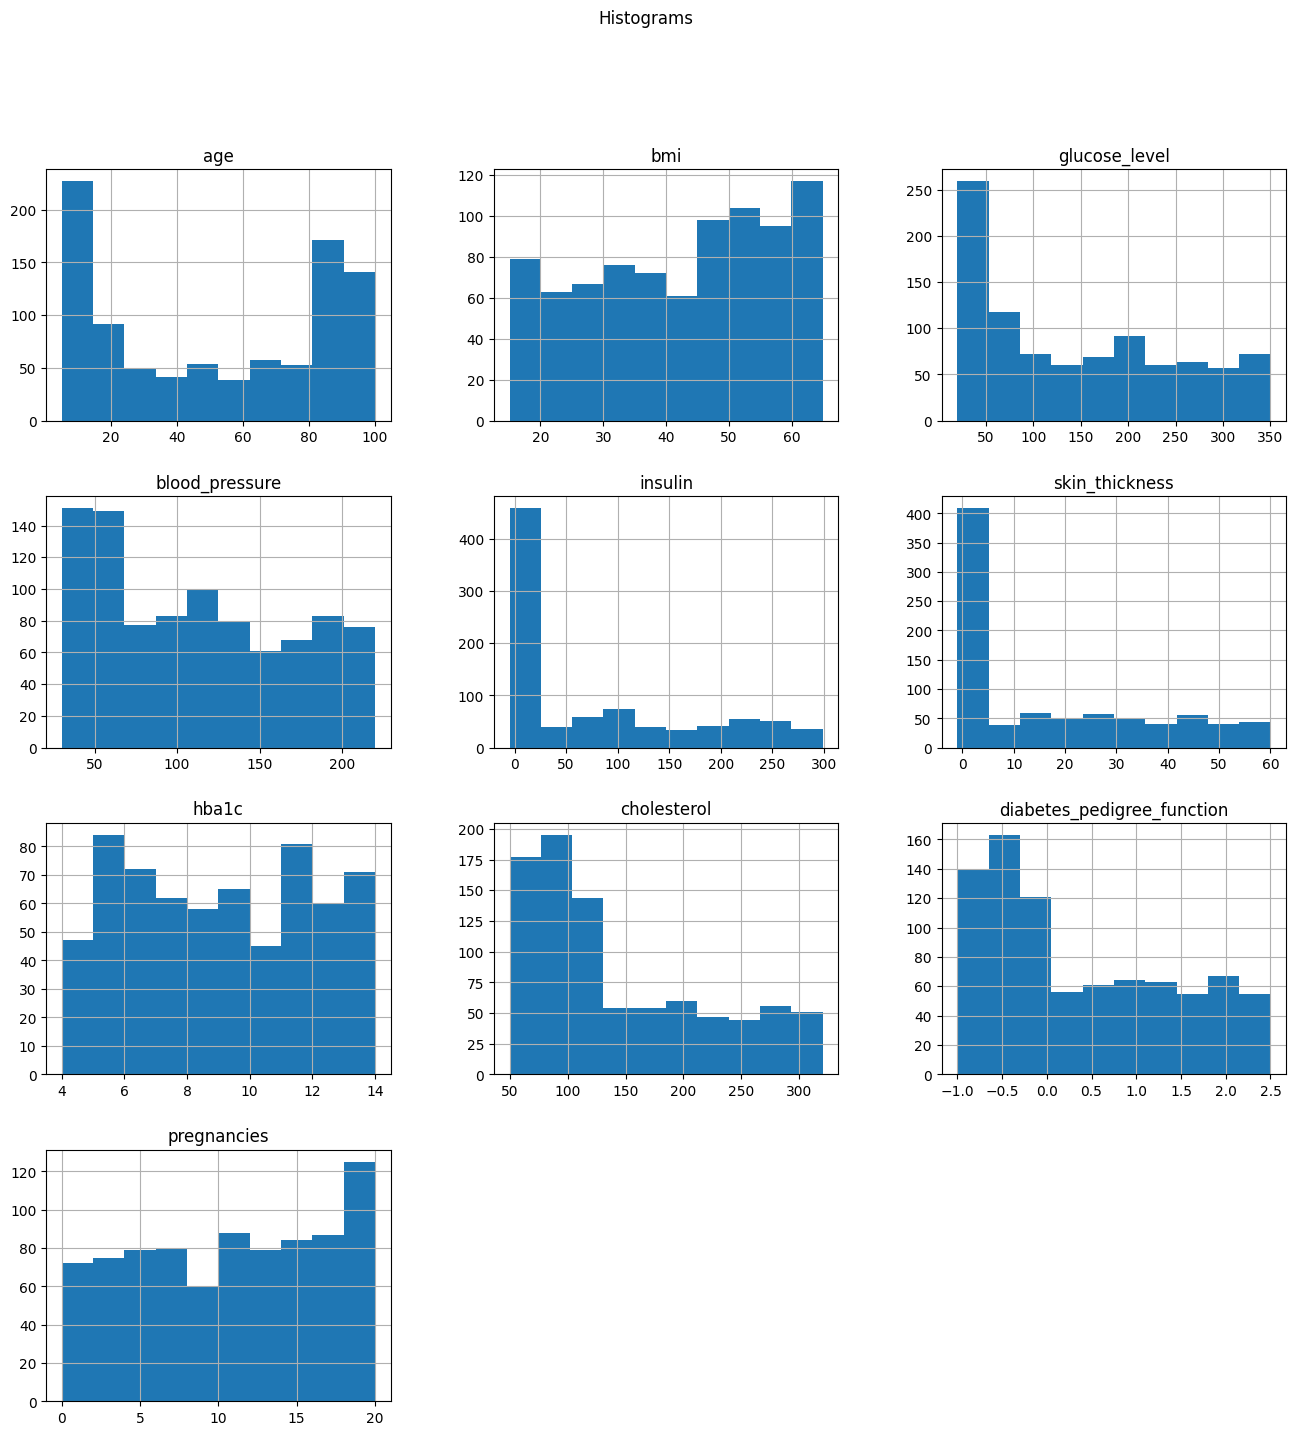
\includegraphics[width=0.4\linewidth]{hist4.png}
\caption{Histogram-Based Distribution of Numerical Features in the Diabetes Prediction Dataset}
\end{figure}
\textbf{Inference:}
The histograms illustrate the distribution of the numerical features, including age, BMI, glucose level, blood pressure, insulin, skin thickness, HbA1c, cholesterol, diabetes pedigree function, and pregnancies.
Several features, such as insulin, skin thickness, and glucose level, exhibit skewed distributions, indicating that patient measurements are not uniformly distributed across the dataset.
The variation in feature distributions suggests that the dataset captures a wide range of patient health characteristics, which can provide valuable information for diabetes prediction.

\vspace{0.5cm}
     \item {\Large\textbf{Iris Dataset}}
\subsection*{Dataset overview :-}
\begin{figure}[H]
\centering
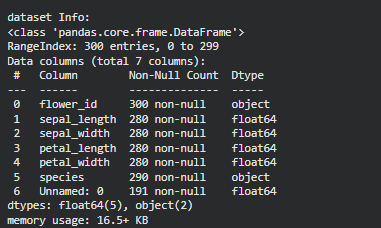
\includegraphics[width=0.4\linewidth]{info5.png}
\caption{Dataset Information Showing Feature Names, Data Types, and Non-Null Values of the Iris Flower Dataset}
\end{figure}
\textbf{Inference:}
The dataset contains 300 records with 7 features, including 5 numerical features and 2 categorical features.
Several attributes, such as sepal\_length, sepal\_width, petal\_length, and petal\_width, contain missing values (280 non-null), while Unnamed: 0 has the highest number of missing values (191 non-null).
The target variable species has 290 non-null values and is categorical (object), indicating that the dataset is suitable for a supervised classification task after handling missing values and encoding categorical features.

\subsection*{Statistical summary}
\begin{figure}[H]
\centering
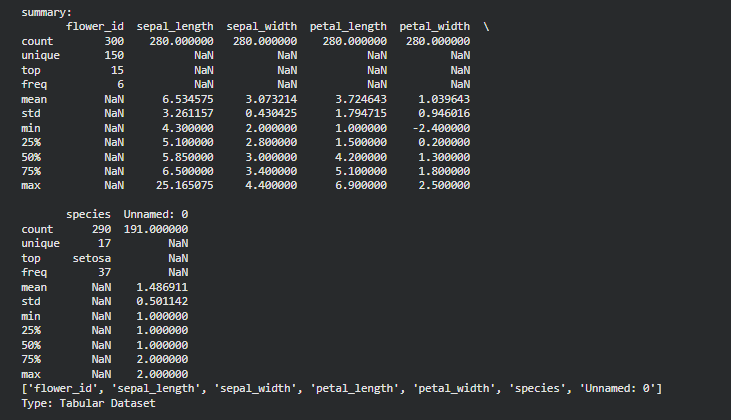
\includegraphics[width=0.4\linewidth]{summary5.png}
\caption{Statistical Summary of the Iris Flower Dataset}
\end{figure}
\textbf{Inference:}
The statistical summary presents descriptive measures such as count, mean, standard deviation, minimum, maximum, and quartiles for the numerical features, along with unique values and frequency for categorical features.
The numerical features (sepal\_length, sepal\_width, petal\_length, and petal\_width) exhibit varying ranges and distributions, indicating differences in flower measurements across the dataset.
The species column contains 17 unique categories, with setosa being the most frequent class, while the reduced counts of several features indicate the presence of missing values that should be handled before model training.

\subsection*{Missing value analysis}
\begin{figure}[H]
\centering
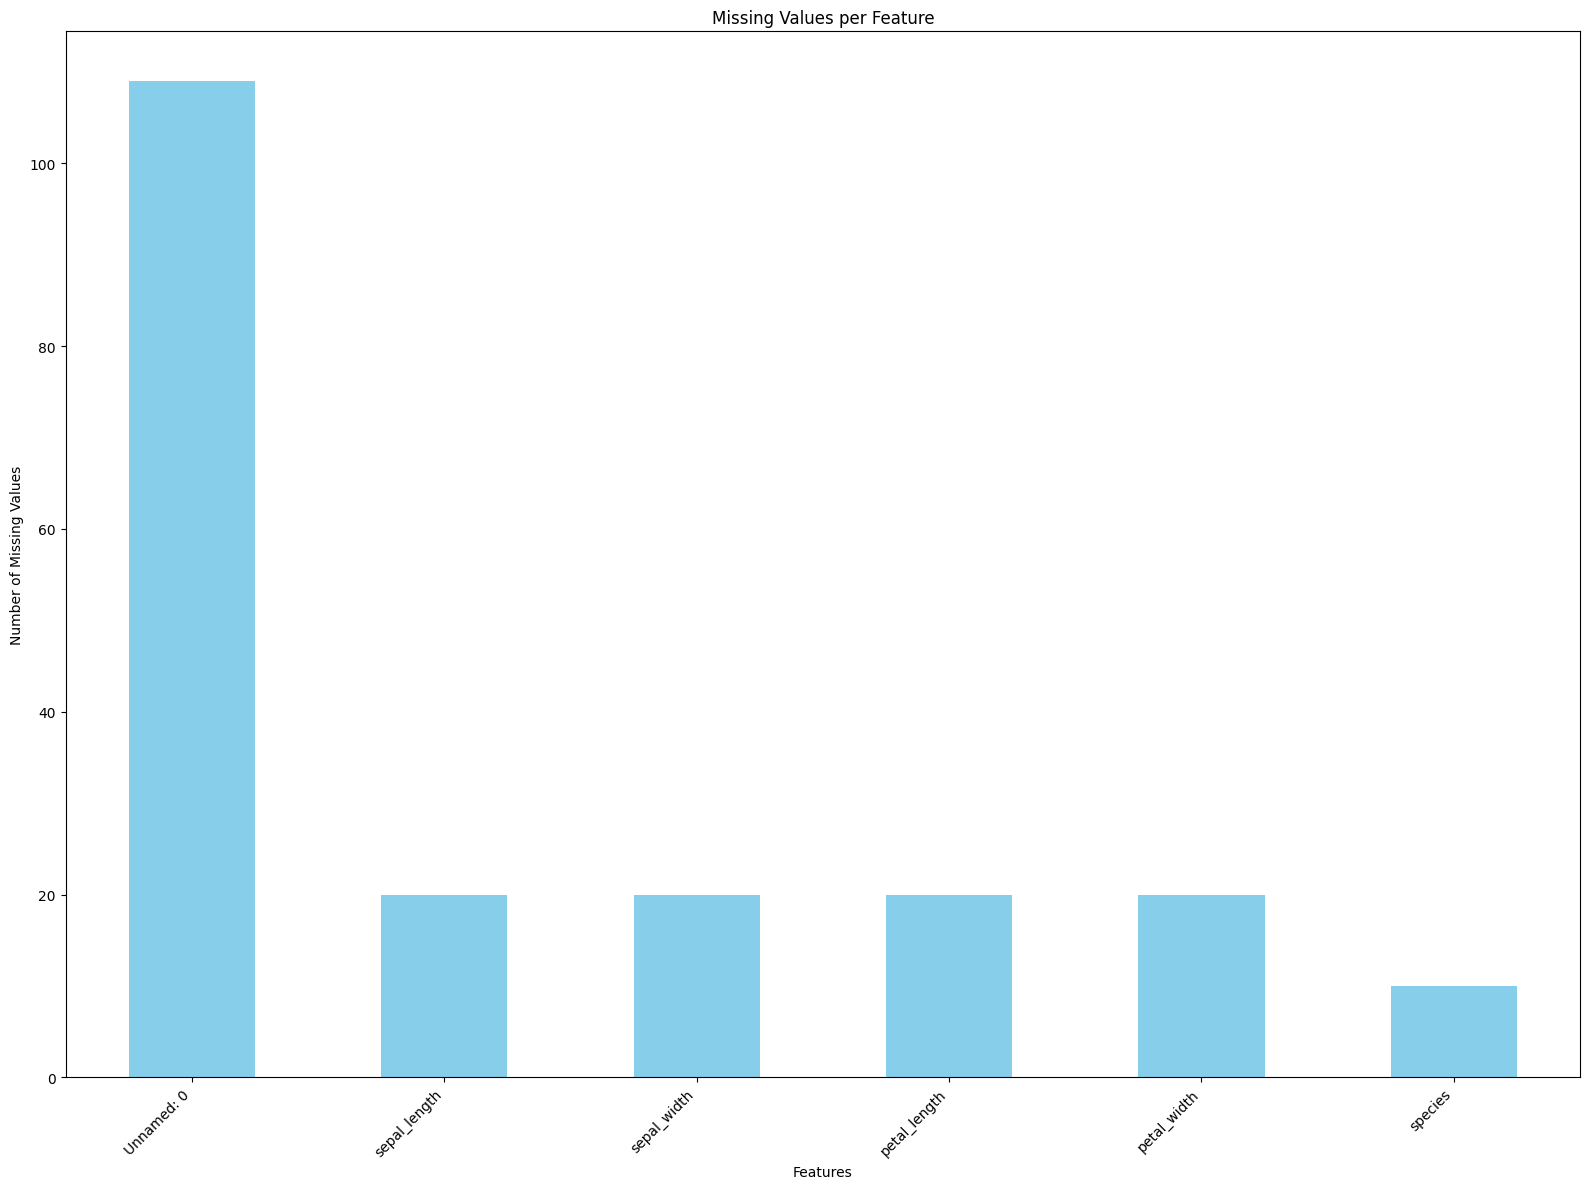
\includegraphics[width=0.4\linewidth]{missing5.png}
\caption{Missing Values Distribution Across Features in the Iris Flower Dataset}
\end{figure}
\textbf{Inference:}
Missing values are present in six features, while flower\_id contains no missing values.
The Unnamed: 0 column has the highest number of missing values (approximately 109), whereas sepal\_length, sepal\_width, petal\_length, and petal\_width each contain about 20 missing values.
The species target column has only 10 missing values, while the remaining missing values should be handled through appropriate imputation before model training.

\subsection*{Class distribution}
\begin{figure}[H]
\centering
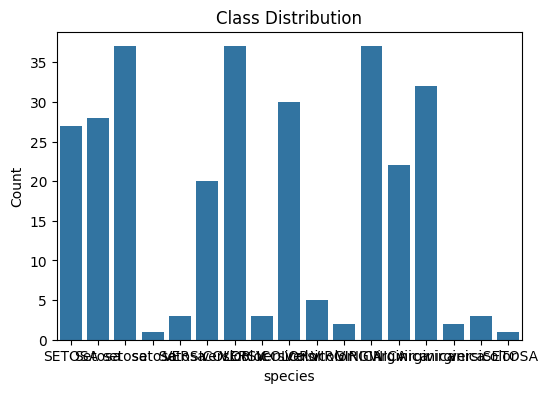
\includegraphics[width=0.4\linewidth]{classd5.png}
\caption{Class Distribution of the Iris Flower Dataset}
\end{figure}
\textbf{Inference:}
The target variable species contains 17 distinct class labels, indicating inconsistent naming and representation of flower species.
The class frequencies vary across categories, with some labels occurring much more frequently than others, resulting in an imbalanced distribution.
Before training a classification model, the class labels should be standardized by merging different representations of the same species (e.g., differences in capitalization or spelling) to obtain consistent target classes.

\subsection*{Correlation matrix}
\begin{figure}[H]
\centering
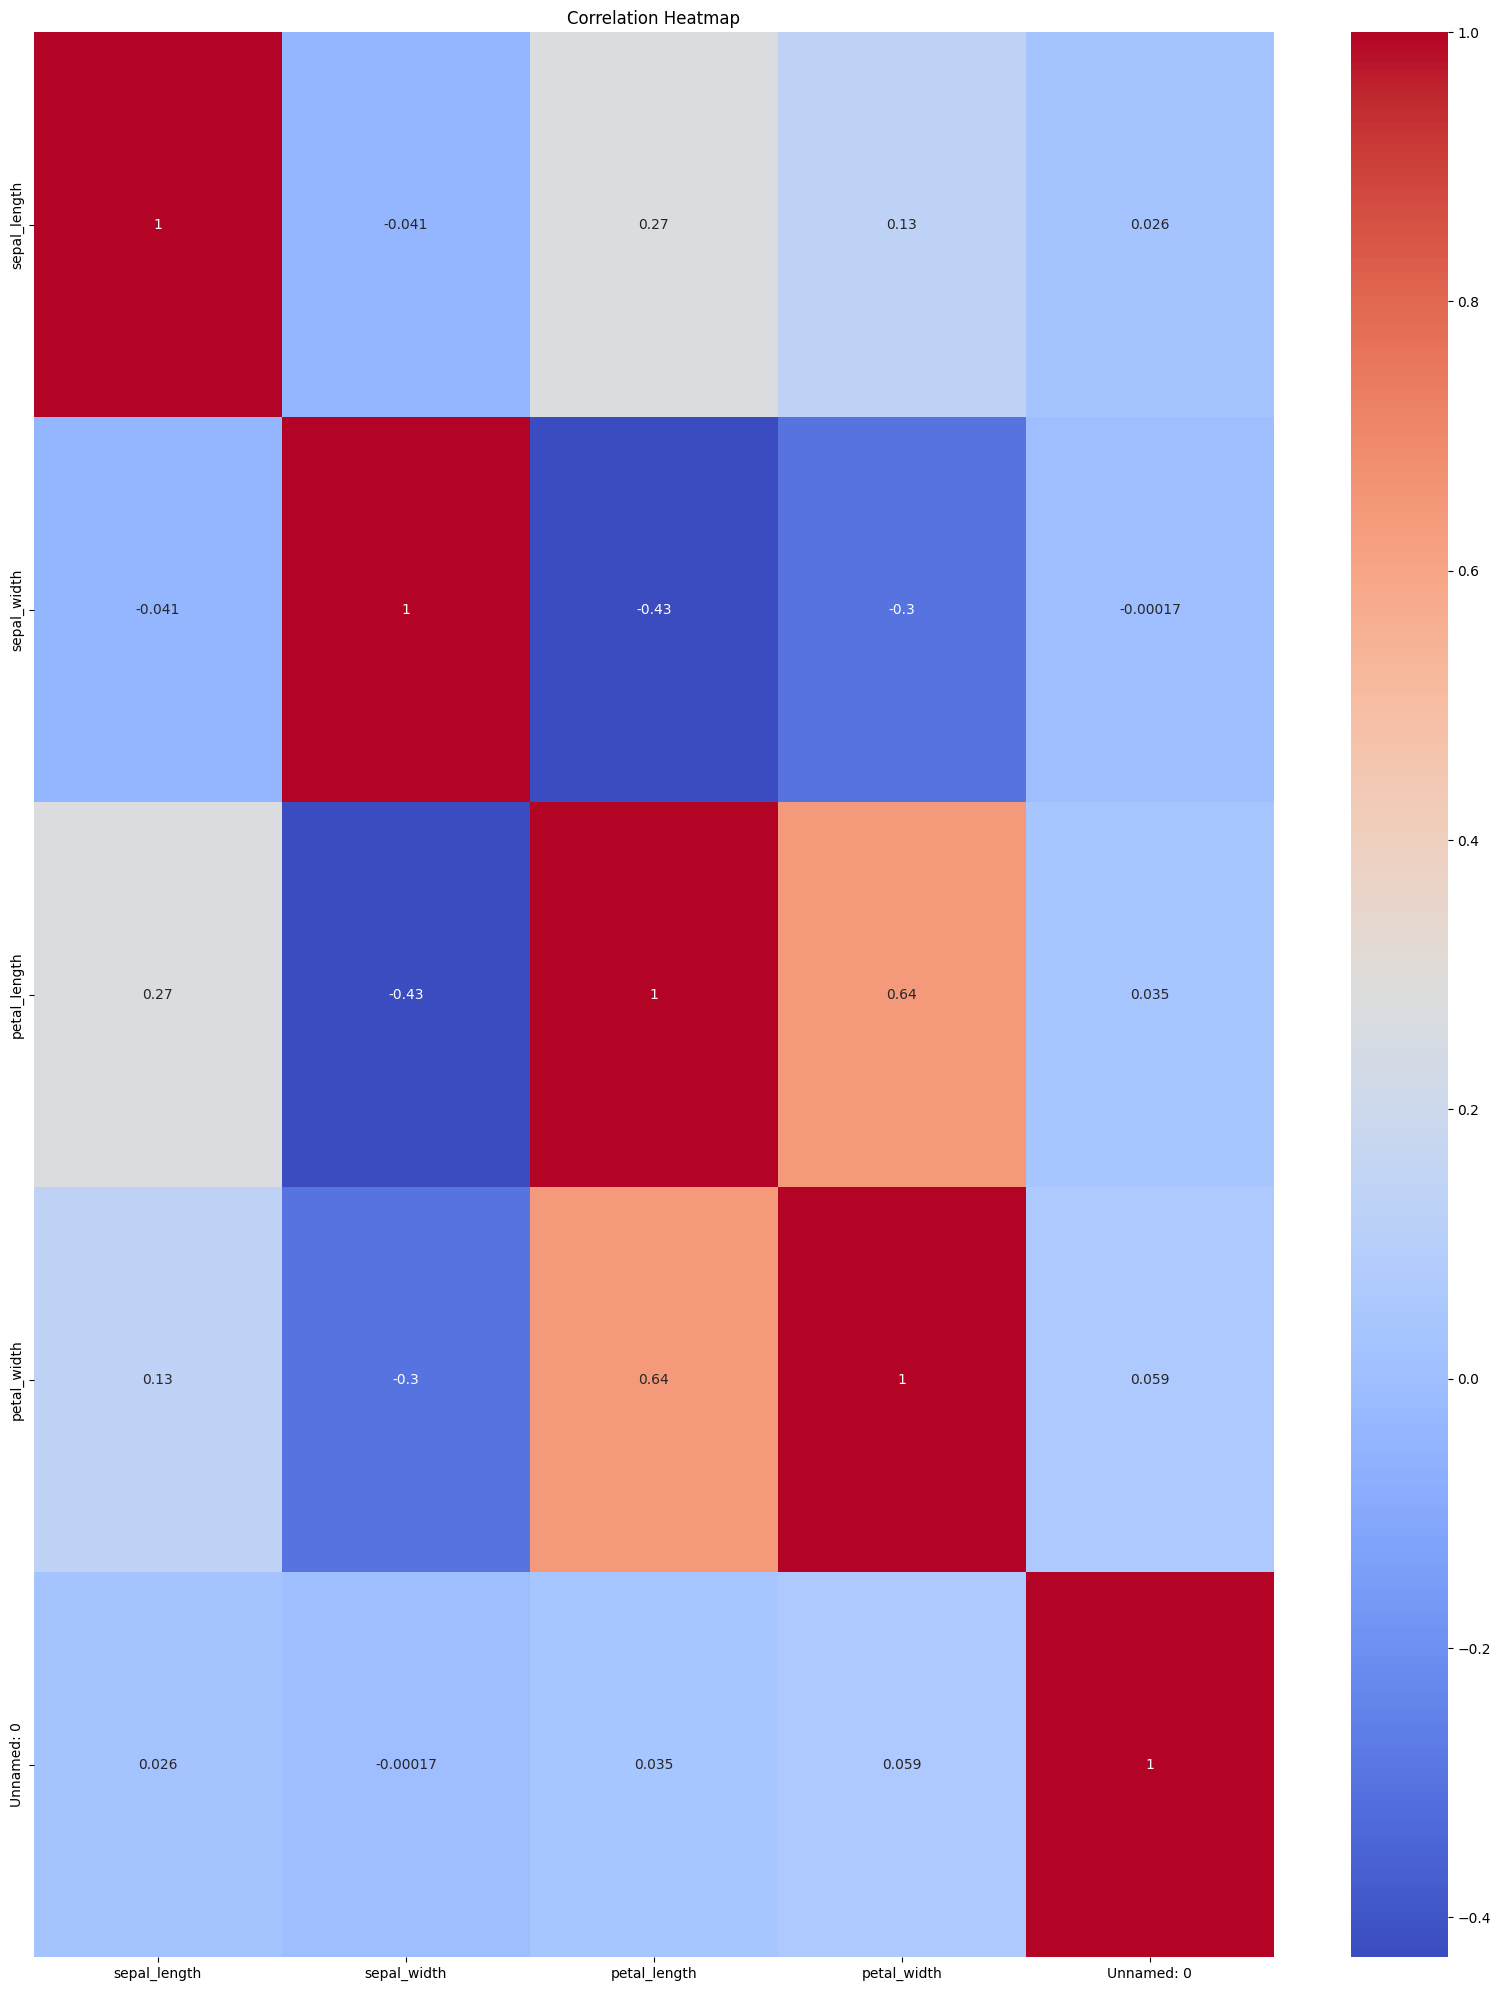
\includegraphics[width=0.4\linewidth]{corr5.png}
\caption{Correlation Heatmap of Numerical Features in the Iris Flower Dataset}
\end{figure}
\textbf{Inference:}
The heatmap shows the pairwise correlations among the numerical features, with diagonal values of 1.0 representing each feature's correlation with itself.
petal\_length and petal\_width exhibit the strongest positive correlation (0.64), indicating that flowers with longer petals tend to have wider petals.
Most other feature pairs show weak to moderate correlations, suggesting that the numerical features capture different aspects of the iris flowers with limited redundancy.

\subsection*{Feature distribution}
\begin{figure}[H]
\centering
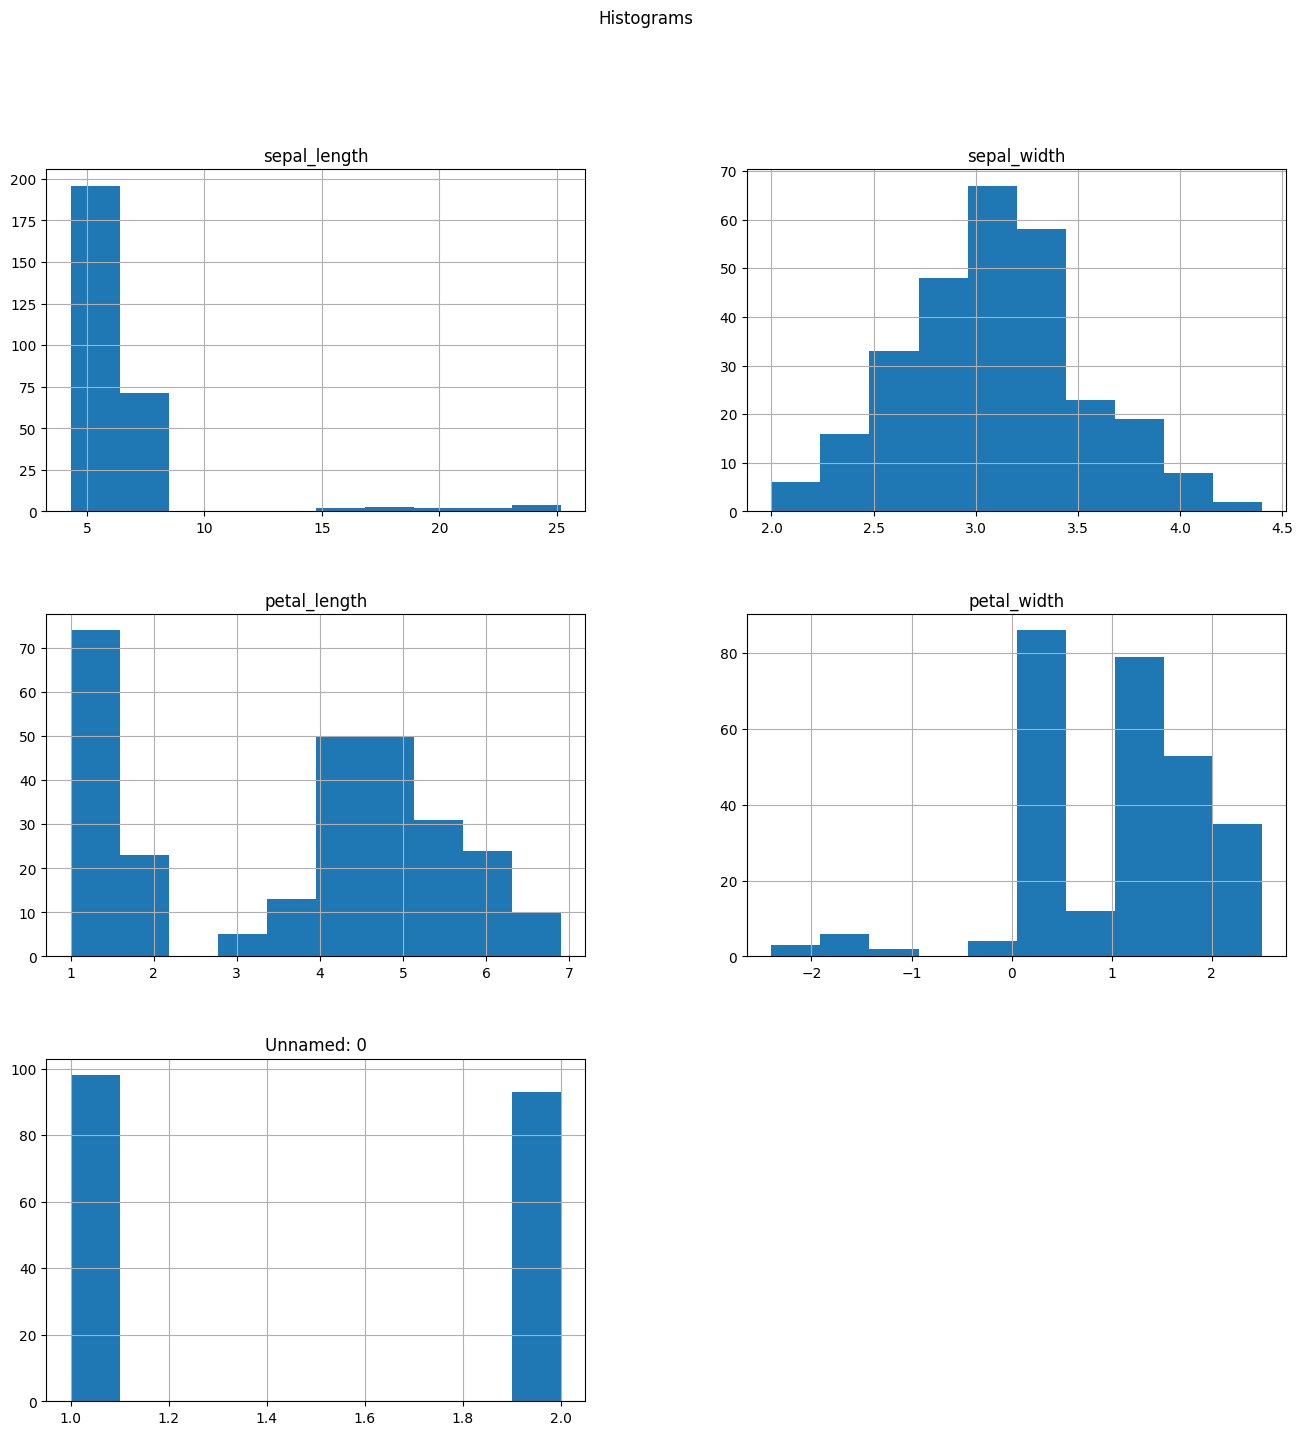
\includegraphics[width=0.4\linewidth]{hist5.png}
\caption{Histogram-Based Distribution of Numerical Features in the Iris Flower Dataset}
\end{figure}
\textbf{Inference:}
The histograms illustrate the distributions of the numerical features, including sepal length, sepal width, petal length, petal width, and Unnamed: 0.The features exhibit different distribution patterns, with sepal width appearing relatively symmetric, while petal length and petal width show greater variation and multiple peaks across observations.
The variation in feature distributions indicates that the flower measurements differ across samples, providing useful characteristics for distinguishing between iris species.
\end{itemize}

\section{Data Preprocessing}
\subsection*{Loan Amount Prediction}
\begin{itemize}
\item Missing value handling:
\begin{itemize}
\item Missing values were identified using df.isnull().sum() and handled before model training.
\item Numerical features were imputed using their mean values, while categorical features were imputed using the mode (most frequent value).
\item This ensured that the dataset contained no missing values and prevented information loss caused by deleting records.
\end{itemize}
\item Encoding
\begin{itemize}
\item Categorical features such as gender, maritalstatus, educationlevel, employmentstatus, loanpurpose, gradesubgrade, and loanpaidback were converted into numerical form using Label Encoding.
\item Encoding transformed categorical values into machine-readable numerical labels while preserving all records for model training.
\end{itemize}
\item Feature scaling
\begin{itemize}
\item Numerical features, including age, annualincome, monthlyincome, loanamount, creditscore, interestrate, totalcreditlimit, and currentbalance, were standardized using StandardScaler.
\item Feature scaling ensures that all numerical variables have a similar scale, preventing features with larger values from dominating the learning process.
\item The target variable (loanpaidback) was excluded from scaling.
\end{itemize}
\item Train-test split
\begin{itemize}
\item The preprocessed dataset was divided into 70\% training, 15\% validation, and 15\% testing sets.
\item Stratified sampling was applied when possible to preserve the class distribution across the subsets. If stratification was not feasible due to insufficient samples in a class, a standard random split was performed.
\end{itemize}
\end{itemize}
\subsection*{ Handwritten character recognition}
\begin{itemize}
\item Missing value handling:
\begin{itemize}
\item missing values were identified using df.isnull().sum() before preprocessing.
\item Only the label column contained missing values (43), while all 64 pixel features and the issue column had no missing values.
\item Records with missing label values were removed, as the target variable is essential for supervised classification.
\end{itemize}
\item Encoding
\begin{itemize}
\item The issue column, being categorical, was encoded into numerical values using Label Encoding to make it suitable for machine learning algorithms.
\item The label column already contained numerical class labels (0–9) and therefore did not require additional encoding.
\item The pixel features were numerical and required no categorical encoding.
\end{itemize}
\item Feature scaling
\begin{itemize}
\item The numerical pixel features were standardized using StandardScaler to ensure a uniform scale across all features.
\item Feature scaling improves the performance of machine learning algorithms by preventing features with larger values from dominating the learning process.
\item The target (label) column was excluded from the scaling process.
\end{itemize}
\item Train-test split
\begin{itemize}
\item The dataset was divided into 618 training samples (70\%), 133 validation samples (15\%), and 133 testing samples (15\%) to ensure reliable model development and evaluation.
\item Each dataset contains 65 input features, while the label column serves as the target variable for supervised classification.
\item The split enables model training on the training set, hyperparameter validation on the validation set, and unbiased performance assessment on the testing set.
\end{itemize}
\end{itemize}
\subsection*{Classification of Email spam and MNIST data}
\begin{itemize}
\item Missing value handling:
\begin{itemize}
\item Missing values in numerical features (num\_links, num\_attachments, message\_length) were replaced using the mean of the respective feature.
\item Missing values in categorical features (email\_id, subject, message, sender, has\_link, contains\_special\_chars, label) were replaced using the mode (most frequent value).
\item This preprocessing step ensured that the dataset contained no missing values before feature selection and model training.
\end{itemize}
\item Encoding
\begin{itemize}
\item Categorical features such as email\_id, subject, message, sender, has\_link, contains\_special\_chars, and label were converted into numerical values using Label Encoding.
\item Label Encoding assigns a unique integer to each distinct category, making the data compatible with machine learning algorithms.
\item The numerical features (num\_links, num\_attachments, and message\_length) were already in numeric form and therefore required no encoding.
\end{itemize}
\item Feature scaling
\begin{itemize}
\item The numerical features (num\_links, num\_attachments, and message\_length) were standardized using StandardScaler.
\item StandardScaler transforms each numerical feature to have a mean of 0 and a standard deviation of 1, ensuring a common scale across all features.
\item Categorical features and the target label were excluded from the scaling process.
\end{itemize}
\item Train-test split
\begin{itemize}
\item The dataset was divided into Training (784 samples), Validation (168 samples), and Testing (169 samples) to support model training, hyperparameter tuning, and performance evaluation.
\item Each sample contains 8 input features, resulting in feature dimensions of (784, 8) for training, (168, 8) for validation, and (169, 8) for testing.
\item Since the label column is the target variable, the dataset was identified as a Supervised Learning Classification problem.
\end{itemize}
\end{itemize}
\subsection*{Predicting Diabetes}
\begin{itemize}
\item Missing value handling:
\begin{itemize}
\item Missing values in numerical features (such as age, BMI, glucose\_level, blood\_pressure, insulin, skin\_thickness, hba1c, cholesterol, diabetes\_pedigree\_function, and pregnancies) were replaced using the mean of their respective columns.
\item Missing values in categorical features (patient\_id, gender, physical\_activity, family\_history, smoking\_status, and diabetes) were replaced using the mode (most frequent value).
\item This imputation process removed all missing values, resulting in a complete dataset suitable for preprocessing, feature selection, and model training.
\end{itemize}
\item Encoding
\begin{itemize}
\item Categorical features such as patient\_id, gender, physical\_activity, family\_history, smoking\_status, and the target variable diabetes were converted into numerical values using Label Encoding.
\item Label Encoding assigns a unique integer to each distinct category, making the categorical data suitable for machine learning algorithms.
\item The remaining features (age, BMI, glucose\_level, blood\_pressure, insulin, skin\_thickness, HbA1c, cholesterol, diabetes\_pedigree\_function, and pregnancies) were already numerical and therefore required no encoding.
\end{itemize}
\item Feature scaling
\begin{itemize}
\item All numerical features (age, BMI, glucose\_level, blood\_pressure, insulin, skin\_thickness, HbA1c, cholesterol, diabetes\_pedigree\_function, and pregnancies) were standardized using StandardScaler.
\item StandardScaler transforms each numerical feature to have a mean of 0 and a standard deviation of 1, ensuring that features with different ranges are placed on a common scale.
\item Categorical features (patient_id, gender, physical_activity, family_history, smoking_status) and the target variable (diabetes) were excluded from the scaling process.
\end{itemize}
\item Train-test split
\begin{itemize}
\item The dataset was divided into Training (718 samples), Validation (154 samples), and Testing (154 samples) to enable model training, validation, and final performance evaluation.
\item Each dataset contains 14 input features, resulting in feature dimensions of (718, 14) for training, (154, 14) for validation, and (154, 14) for testing.
\item The diabetes column was selected as the target variable, identifying the problem as a Supervised Learning – Classification task.
\end{itemize}
\end{itemize}
\subsection*{Iris Dataset}
\begin{itemize}
\item Missing value handling:
\begin{itemize}
\item Missing values in the numerical features (sepal\_length, sepal\_width, petal\_length, petal\_width, and Unnamed: 0) were replaced using the mean of their respective columns.
\item Missing values in the categorical feature (species) were replaced using the mode (most frequent class), while flower\_id required no imputation since it contained no missing values.
\item This imputation process eliminated all missing values, resulting in a complete dataset for subsequent preprocessing, feature selection, and classification.
\end{itemize}
\item Encoding
\begin{itemize}
\item The categorical features flower\_id and species were converted into numerical values using Label Encoding.
\item Label Encoding assigns a unique integer to each distinct category, enabling machine learning algorithms to process categorical data.
\item The remaining features (sepal\_length, sepal\_width, petal\_length, petal\_width, and Unnamed: 0) were already numerical and therefore required no encoding.
\end{itemize}
\item Feature scaling
\begin{itemize}
\item The numerical features (sepal\_length, sepal\_width, petal\_length, petal\_width, and Unnamed: 0) were standardized using StandardScaler.
\item StandardScaler transforms each numerical feature to have a mean of 0 and a standard deviation of 1, ensuring that all features are on a common scale.
\item The categorical features (flower\_id and species) were excluded from the scaling process after being encoded using Label Encoding.
\end{itemize}
\item Train-test split
\begin{itemize}
\item The dataset was divided into Training (193 samples), Validation (42 samples), and Testing (42 samples) for model training, validation, and performance evaluation.
\item Each sample consists of 4 input features, resulting in feature dimensions of (193, 4) for training, (42, 4) for validation, and (42, 4) for testing.
\item Since some species classes contained fewer than 2 samples, the dataset was split without stratification. The species column was selected as the target variable, identifying the problem as a Supervised Learning – Classification task.
\end{itemize}
\end{itemize}

\section{Experimental Setup}
\begin{tabular}{ll}
\toprule
Python Version & 3.14.0\\
Scikit-Learn Version & 1.6.1\\
IDE & Google Colab\\
Operating System & Windows\\
Hardware & Laptop\\
\bottomrule
\end{tabular}

\section{Discussion}
\begin{itemize}
\item Observation:
Exploratory Data Analysis revealed variations in feature distributions, missing values, and class distributions across datasets, highlighting the importance of dataset-specific preprocessing before model development.
\item Strength:
A common machine learning pipeline was successfully applied to multiple datasets with minimal modifications.
\item Limitation:
Different dataset types (tabular, text, and image) require specialized preprocessing techniques, which are not fully handled by a single generic pipeline.
\item Improvement:
The pipeline can be enhanced by incorporating dataset-specific preprocessing methods, feature engineering, and hyperparameter optimization to improve overall performance.
\end{itemize}

\section{Conclusion}
The experiment successfully implemented a complete machine learning pipeline for multiple datasets, including dataset analysis, preprocessing, feature selection, data splitting, and model evaluation. Exploratory Data Analysis helped identify data characteristics such as missing values, feature distributions, and correlations, while preprocessing techniques prepared the data for machine learning. The study demonstrated that different datasets require different preprocessing strategies depending on their type (tabular, text, or image metadata), highlighting the importance of selecting appropriate techniques for accurate and reliable model development.

\section{References}
Datasets :  \url{https://www.kaggle.com/}
\\ IDE : \url{https://colab.research.google.com/}

\end{document}
